\section{Prinzipien der komplexen FM-Synthese}
\label{PrinzipKomplexFM}

Die bisherige Darstellung der Soundsynthese durch Frequenzmodulation (FM) hat sich auf die \textit{einfache} FM konzentriert, d.h. auf die Modulation eines einzelnen Trägers durch einen einzigen Modulator. Dadurch konnten die Prinzipien der Einflussnahme auf die Sounderzeugung über die Parameter von Trägerfrequenz, Modulationsfrequenz sowie den Modulationsindex analytisch klar isoliert werden. In der Praxis ist diese Limitation nicht notwendig, so dass zur Erzeugung komplexer Klangspektren auf den gleichzeitigen Einsatz mehrerer Träger und Modulatoren zurückgegriffen wird. Diese können dabei flexibel miteinander verschaltet werden. Man spricht in diesem Zusammenhang von der \textit{komplexen} FM. Im Folgenden werden die Prinzipien der komplexen FM näher beleuchtet. Auch hier wird zunächst mit einer künstlichen Limitation gearbeitet und der bisher betrachtete Fall entweder um einen weiteren Träger erweitert oder um einen weiteren Modulator. Denkbar sind unter diesen Bedingungen zwei grundsätzliche Verschaltungsmuster, und zwar zum einen eine Parallelschaltung, zum anderen eine Reihenschaltung. Als spezielle Form der Reihenschaltung kann die Rückkopplung des Trägersignals auf sich selbst gesehen werden; dieser Fall der Feedback-Schaltung wird ebenfalls vorgestellt. 

\subsection{Parallelschaltung}

\subsubsection{Parallele Träger mit jeweils eigenem unabhängigen Modulator}

Zur Vollständigkeit soll die simpelste Erweiterung der einfachen FM nicht unerwähnt bleiben, und zwar die Situation zweier paralleler Träger, denen je ein eigener Modulator zugeordnet ist (Abb 1). Dabei handelt es sich streng genommen noch um keine komplexe FM, da die Signalpfade beider Träger erst auf der Ebene des Gesamtausgangssignals gemischt werden und sich ansonsten nicht weiter beeinflussen. Jedes Träger-Modulator-Paar, also $T1$ mit $M1$ sowie $T2$ mit $M2$, folgt dabei für sich genommen den Prinzipien der einfachen FM, so dass für jedes Paar die Lage der Seitenfrequenzbänder gesondert bestimmt und addiert werden kann, womit sich das Ausgangssignal $T1<M1 + T2<M2$ insgesamt ergibt. Lage und Amplitude der Seitenfrequenzbänder folgen direkt aus der gewählten Funktion für die Frequenzmodulation, auch wenn die Herleitung nichttrivial ist und Kenntnis der Eigenschaften der Besselfunktion voraussetzt. 

Alle Spektren und Wellenformen in diesem Kapitel der Seminararbeit wurden auf Basis folgender Funktion für die FM modelliert. Auf einen Koeffizienten $A$, der üblicherweise für die Amplitude des gesamten Ausgangssignals vorne auf die Funktion aufmultipliziert wird, wird im Lauf der folgenden Ausführungen für verbesserte Übersichtlichkeit verzichtet:
\label{matze:simplefm}
\begin{equation} \label{eq:SimpleFM}
f_{FM}(t) = \sin(w_ct + I\sin(w_mt)) \quad \text{mit} \quad w_ct \quad \text{als Träger-} \quad \text{und} \quad w_mt \quad \text{als Modulationsfreq.}
\end{equation}
Um eine Funktion für das Frequenzspektrum zu erhalten, expandiert man diese über das trigonometrische Additionstheorem \begin{math} \sin(a + b) = \sin(a)\cos(b)+\cos(a)\sin(b) \end{math} und erhält
\begin{equation}\label{eq:BesselZwischenform}
\sin(w_ct + I\sin(w_mt)) = \sin(w_ct)\cos(I\sin(w_mt)) + \cos(w_ct)\sin(I\sin(w_mt)).
\end{equation}
Die inneren Terme \begin{math} \cos(I\sin(w_mt)) \end{math} und \begin{math} \sin(I\sin(w_mt)) \end{math} können nun über die Besselfunktion wie folgt ausgedrückt werden. Die Herleitung geschieht über die Erzeugerfunktion; siehe \cite[S.361, Satz~9.1.42 und Satz~9.1.43]{abramowitz}:
\begin{equation}\label{eq:Besselsin}
\sin(I\sin(w_mt)) = 2J_1(I)\sin(w_mt)+2J_3(I)\sin(3w_mt)+...+2J_{2n+1}(I)\sin((2n+1)w_mt)+...
\end{equation}
\begin{equation}\label{eq:Besselcos}
\cos(I\sin(w_mt)) = J_0(I)+2J_2(I)\cos(2w_mt)+...+2J_{2n}(I)\cos(2nw_mt)+...
\end{equation}
Man setzt dies in \ref{eq:BesselZwischenform} ein und expandiert alle auftretende Terme der Form \begin{math} \sin(w_ct)\cos(2nw_mt) \end{math} über das Additionstheorem \begin{math} \sin(a)\cos(b) = \frac{1}{2}\left(\sin(x+y)+\sin(x-y)\right) \end{math} sowie alle Terme der Form \begin{math} \cos(w_ct)\sin((2n+1)w_mt) \end{math} über  \begin{math} \cos(a)\sin(b) = \frac{1}{2}\left(\sin(x+y)-\sin(x-y)\right) \end{math}. Letztlich gilt: 
\begin{equation}
\begin{split}
\sin(w_ct + I\sin(w_mt)) \\ &\quad = J_0(I)\sin(w_ct) \\ &\quad + J_1(I)(\sin(w_ct + w_mt) - \sin(w_ct - w_mt)) \\ &\quad + J_2(I)(\sin(w_ct + 2w_mt)+\sin(w_ct-2w_mt)) \\ &\quad  + J_3(I)(\sin(w_ct + 3w_mt) - \sin(w_ct - 3w_mt)) \\ &\quad  + ...
\end{split}
\end{equation}
(\cite[S.528]{chowningPaper}). Zieht man die Besselkoeffizienten in die Klammer, lässt sich die Lage der Seitenfrequenzbänder bereits aus der Funktion auslesen:
\begin{equation}\label{eq:FormelinchenBessel}
\begin{split}
\sin(w_ct + I\sin(w_mt)) \\ &\quad = J_0(I)\sin(w_ct) \\ &\quad + J_1(I)\sin(w_ct + w_mt) \quad\enspace - J_1(I)\sin(w_ct - w_mt) \\ &\quad + J_2(I)\sin(w_ct + 2w_mt) \quad + J_2(I)\sin(w_ct-2w_mt) \\ &\quad  + J_3(I)\sin(w_ct + 3w_mt) \quad - J_3(I)\sin(w_ct - 3w_mt) \\ &\quad  + ...
\end{split}
\end{equation}
Die erste Zeile zeigt hier die Lage der Trägerfrequenz an, während jede folgende Zeile stets die Lage eines oberen Seitenbands angibt (erster Term) sowie das dazugehörige untere Seitenband (zweiter Term). 

Man kann in dieser Darstellung am Vorzeichen des jeweiligen Terms ablesen, dass Besselkoeffizienten ungerader Ordnung zu negativen Amplitudenwerten des jeweiligen unteren Seitenbandes führen. Da negative Frequenzen einer Phasenverschiebung um 180 Grad entsprechen, erhält man die endgültigen, akustisch wahrgenommenen Frequenzen durch die Spiegelung der negativen Frequenzen je einmal an Abszisse und Ordinate. Dies enspricht einer Phasenverschiebung (Spiegelung Abszisse) im positiven Bereich (Spiegelung Ordinate). Dabei kann es natürlich zur Auslöschung oder Verstärkung von Bändern durch die Addition ursprünglich negativer Frequenzbänder auf bereits vorhandene im positiven Bereich kommen. 

Die Funktion \ref{eq:FormelinchenBessel} kann übersichtlich zusammengefasst werden (\cite{schottstaedtWeb}) zu 
\begin{equation}\label{esq:Besselbabymonster}
\sin(w_ct + I\sin(w_mt)) = \sum_{n=-\infty}^{\infty}J_n(I)\sin(w_ct+nw_mt)
\end{equation}
Das Frequenzspektrum für die einfache FM weist nun im positiven als auch im negativen Bereich stets im Abstand \begin{math} w_m \end{math} um die Trägerfrequenz \begin{math} w_c \end{math} Seitenbänder auf. Die jeweiligen Amplituden werden dabei durch die Ordnung der Besselfunktion bestimmt in Abhängigkeit vom Modulationsindex, welcher als Argument an die Besselfunktion übergeben wird. Die Besselfunktion liefert dabei ab einem Modulationsindex größer ca. 2,5 auch negative Vorzeichen für die Seitenfrequenzen zurück, wie folgende grafischen Darstellung der Besselfunktion nach den Parametern Modulationsindex und Nummer des Seitenbands zeigt: \ref{fig:bessel3D}. Die für beide Paare $T1<M1 + T2<M2$ so ermittelten Frequenzspektren können für diese Form der Parallelschaltung in einem abschließenden Schritt einfach addiert werden und liefern so das gesamte Frequenzspektrum des gemischten Ausgangssignals. 

Dies lässt sich in MATLAB komfortabel visualisieren. Zunächst das erste Paar T1 und M1:
\FloatBarrier
\begin{figure} [ht]
\centering
  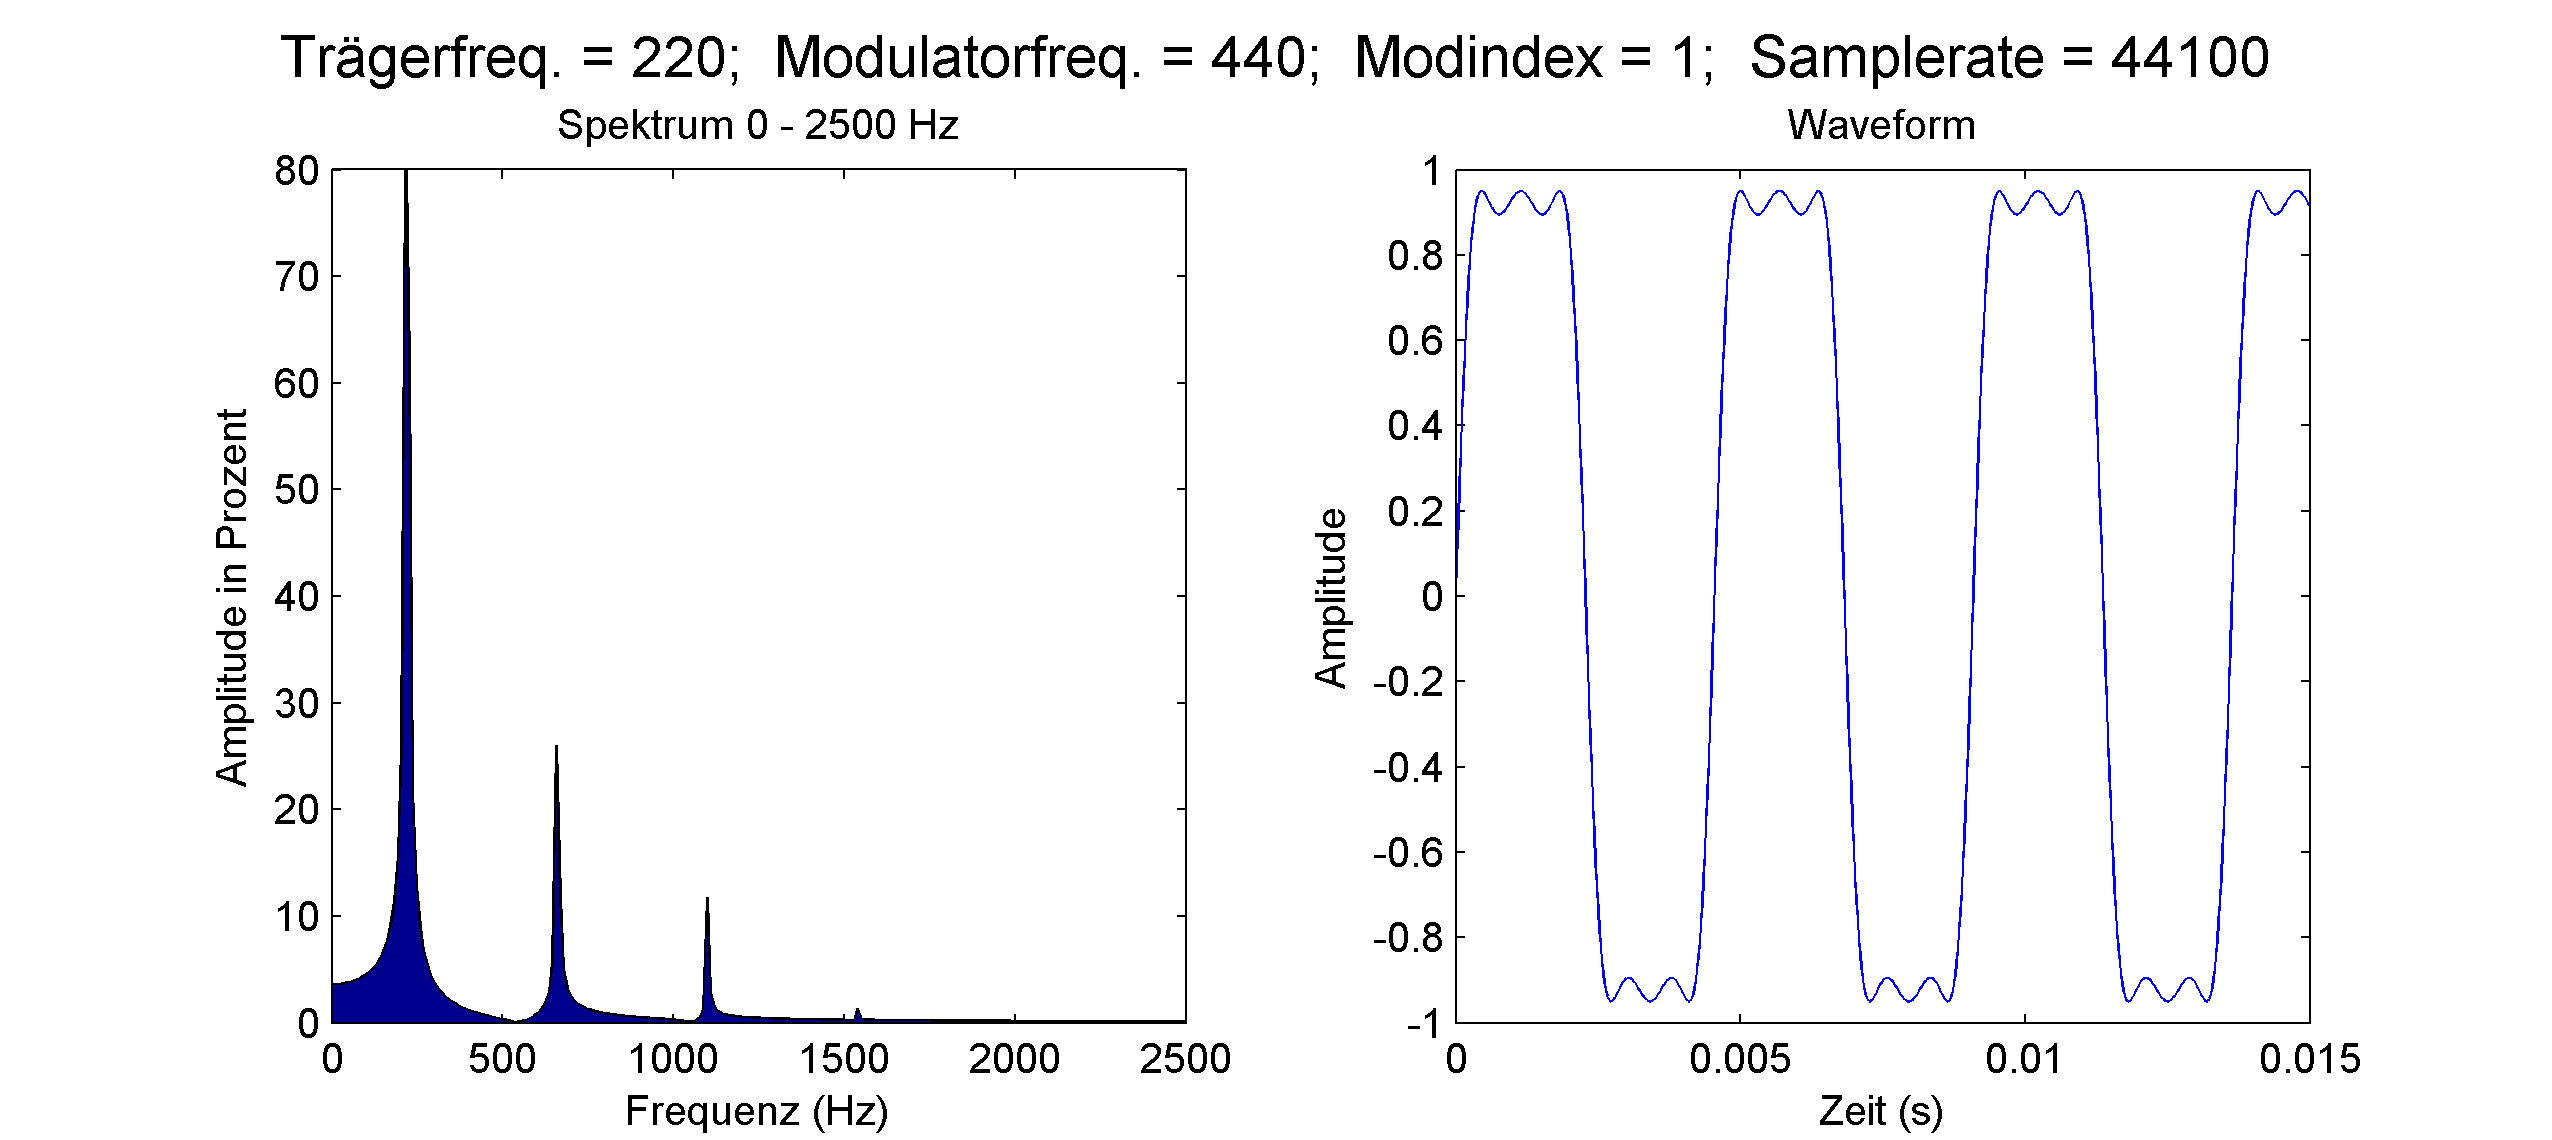
\includegraphics[width=0.95\textwidth]{parT1M1.png}
\caption{Einfache FM mit $f_c = 220$, $w_m = 440$, $I = 1$. }
Quelle: Eigene Darstellung in MATLAB
\end{figure}
\FloatBarrier
Hier das Spektrum für T2 und M2:
\FloatBarrier
\begin{figure} [ht]
\centering
  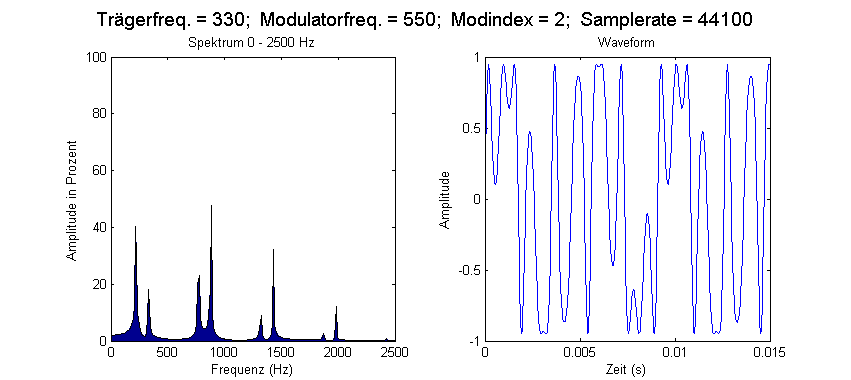
\includegraphics[width=0.95\textwidth]{parT2M2.png}
\caption{Einfache FM mit $f_c = 330$, $w_m = 550$, $I = 2$. }
Quelle: Eigene Darstellung in MATLAB
\end{figure}
\FloatBarrier
Bei den Spektren für beide einfachen FM sieht man sehr gut, dass sich die Seitenfrequenzbänder in Abständen der Modulationsfrequenz um die Trägerfrequenz nach beiden Seiten hin ausbreiten.

Abschließend das Spektrum für die Parallelschaltung beider Träger-Modulator-Paare. Man sieht sehr gut, dass sich die Einzelspektren aus den beiden Plots oben aufaddieren: 
\FloatBarrier
\begin{figure} [ht]
\centering
  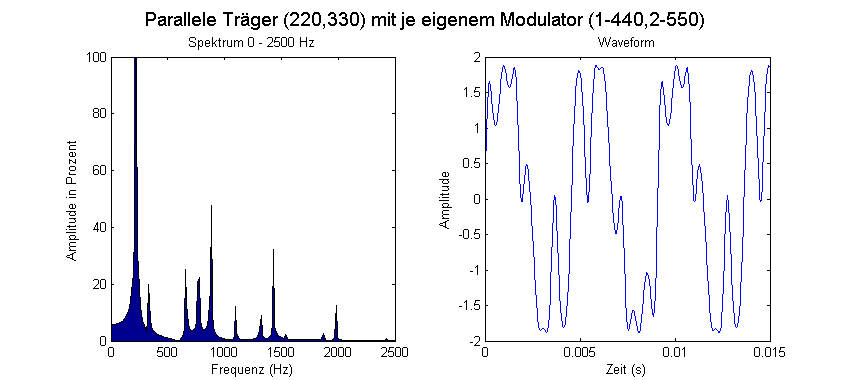
\includegraphics[width=0.95\textwidth]{parT1M1T2M2.png}
\caption{Parallele FM mit $f_{c1} = 220$, $f_{c2} = 330$, $w_{m1} = 440$, $w_{m2} = 550$, $I_1 = 1$, $I_2 = 2$. }
Quelle: Eigene Darstellung in MATLAB
\end{figure}
\FloatBarrier

\subsubsection{Parallele Träger mit einem gemeinsamen Modulator}

Teilen sich zwei Träger $T1$ und $T2$ denselben Modulator $M$, kann das Frequenzspektrum ebenfalls als Summe zweier unabhängiger einfacher FM betrachtet werden. Hierzu berechnet man zunächst das Frequenzspektrum des einen Trägers $T1$ anhand Modulationsfrequenz und dem -index des Modulators M. Anschließend berechnet man das Frequenzspektrum für den zweiten Träger $T2$, wobei wieder Frequenz und Modulationsindex von Modulator $M$ bezogen werden. Aufsummiert ergibt sich das Gesamtspektrum. Das Interessante an dieser Form der Parallelschaltung besteht in der Möglichkeit, nur einen einzigen Modulator zur Modulation mehrerer vorhandener Träger, deren Modulatoren dieselbe Modulationsfrequenz aufweisen, zu verwenden. Dadurch können die freigewordenen Modulatoren für andere Zwecke verwendet werden, z.B. um einen der Träger durch zwei Modulatoren zu modulieren (siehe \ref{singlecarryparallelmod} oder sogar zum Modulieren des bereits eingesetzten Modulators (was dann der Kaskadenschaltung entspräche, siehe \ref{cascade}).  

Die Möglichkeit, denselben Modulator für verschiedene Träger zu verwenden, bedeutet logischerweise, dass die \textit{individuelle} Modulierbarkeit beider Träger aufgegeben wird, da sich Änderungen an den Einstellungen von $M$ nun zwangsläufig sowohl auf $T1$ als auch auf $T2$ auswirken. Die gleiche Mächtigkeit zweier paralleler Träger mit demselben Modulator $M$ im Vergleich zum Setup mit mehreren Trägern, welche jeweils ihren eigenen Modulator mit denselben Einstellungen wie $M$ besitzen, sei im Folgenden illustriert. 

Zunächst das Spektrum zweier Träger, die jeweils von eigenen Modulatoren mit gleichen Einstellungen moduliert werden. Zuerst für den einen Träger:
\FloatBarrier
\begin{figure} [ht]
\centering
  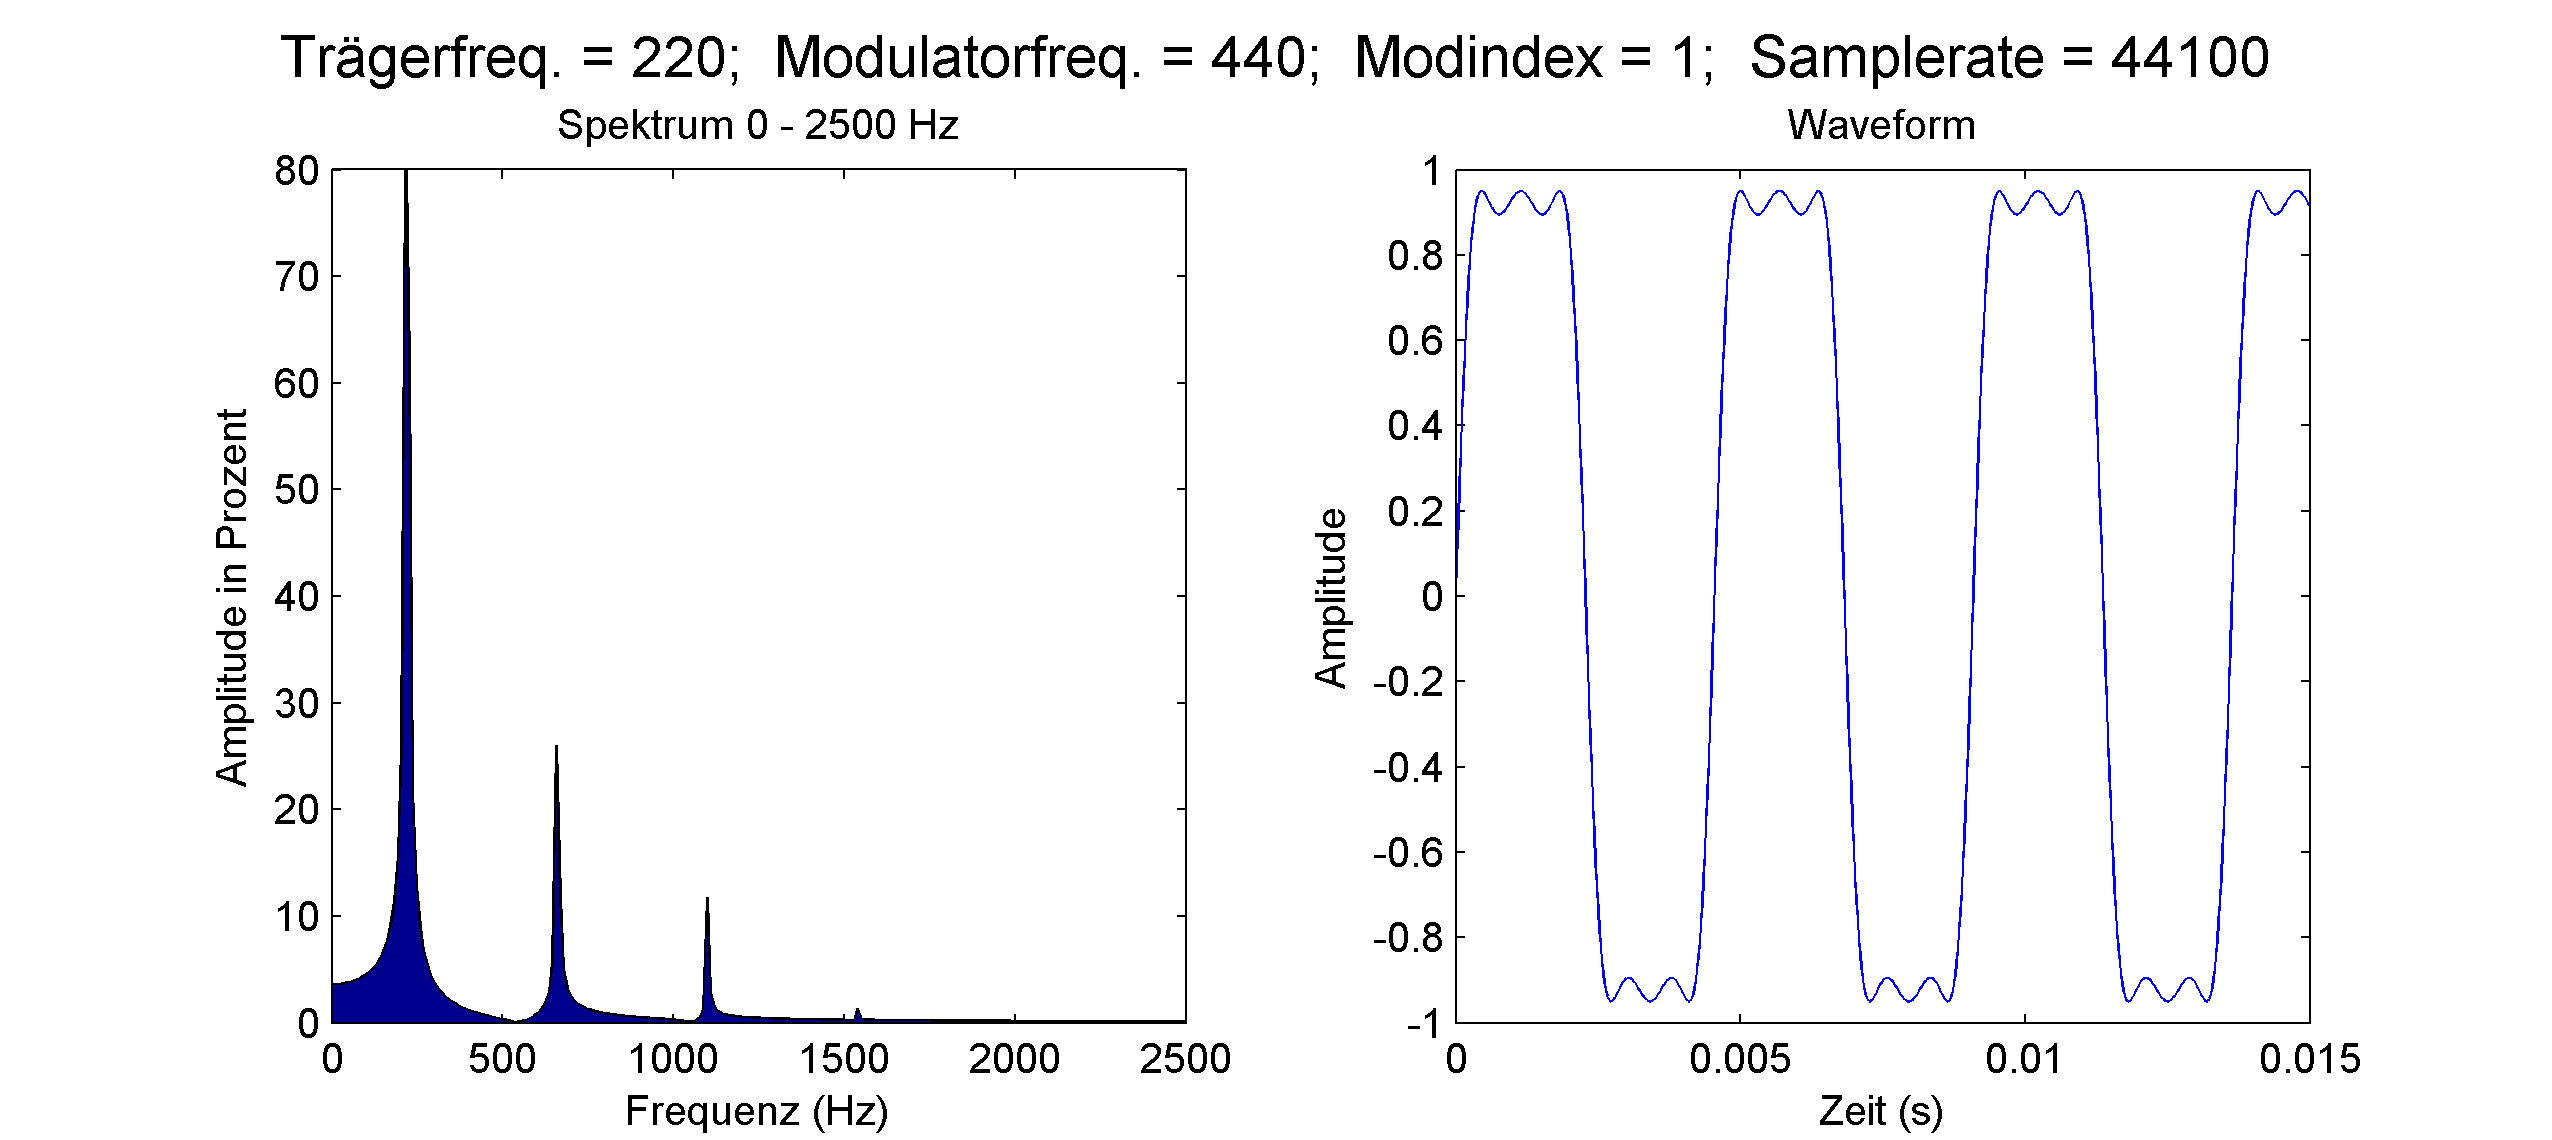
\includegraphics[width=0.95\textwidth]{parT1M1.png}
\caption{Einfache FM mit $f_c = 220$, $w_m = 440$, $I = 1$. }
Quelle: Eigene Darstellung in MATLAB
\end{figure}
\FloatBarrier
Nun für den zweiten Träger:
\FloatBarrier
\begin{figure} [ht]
\centering
  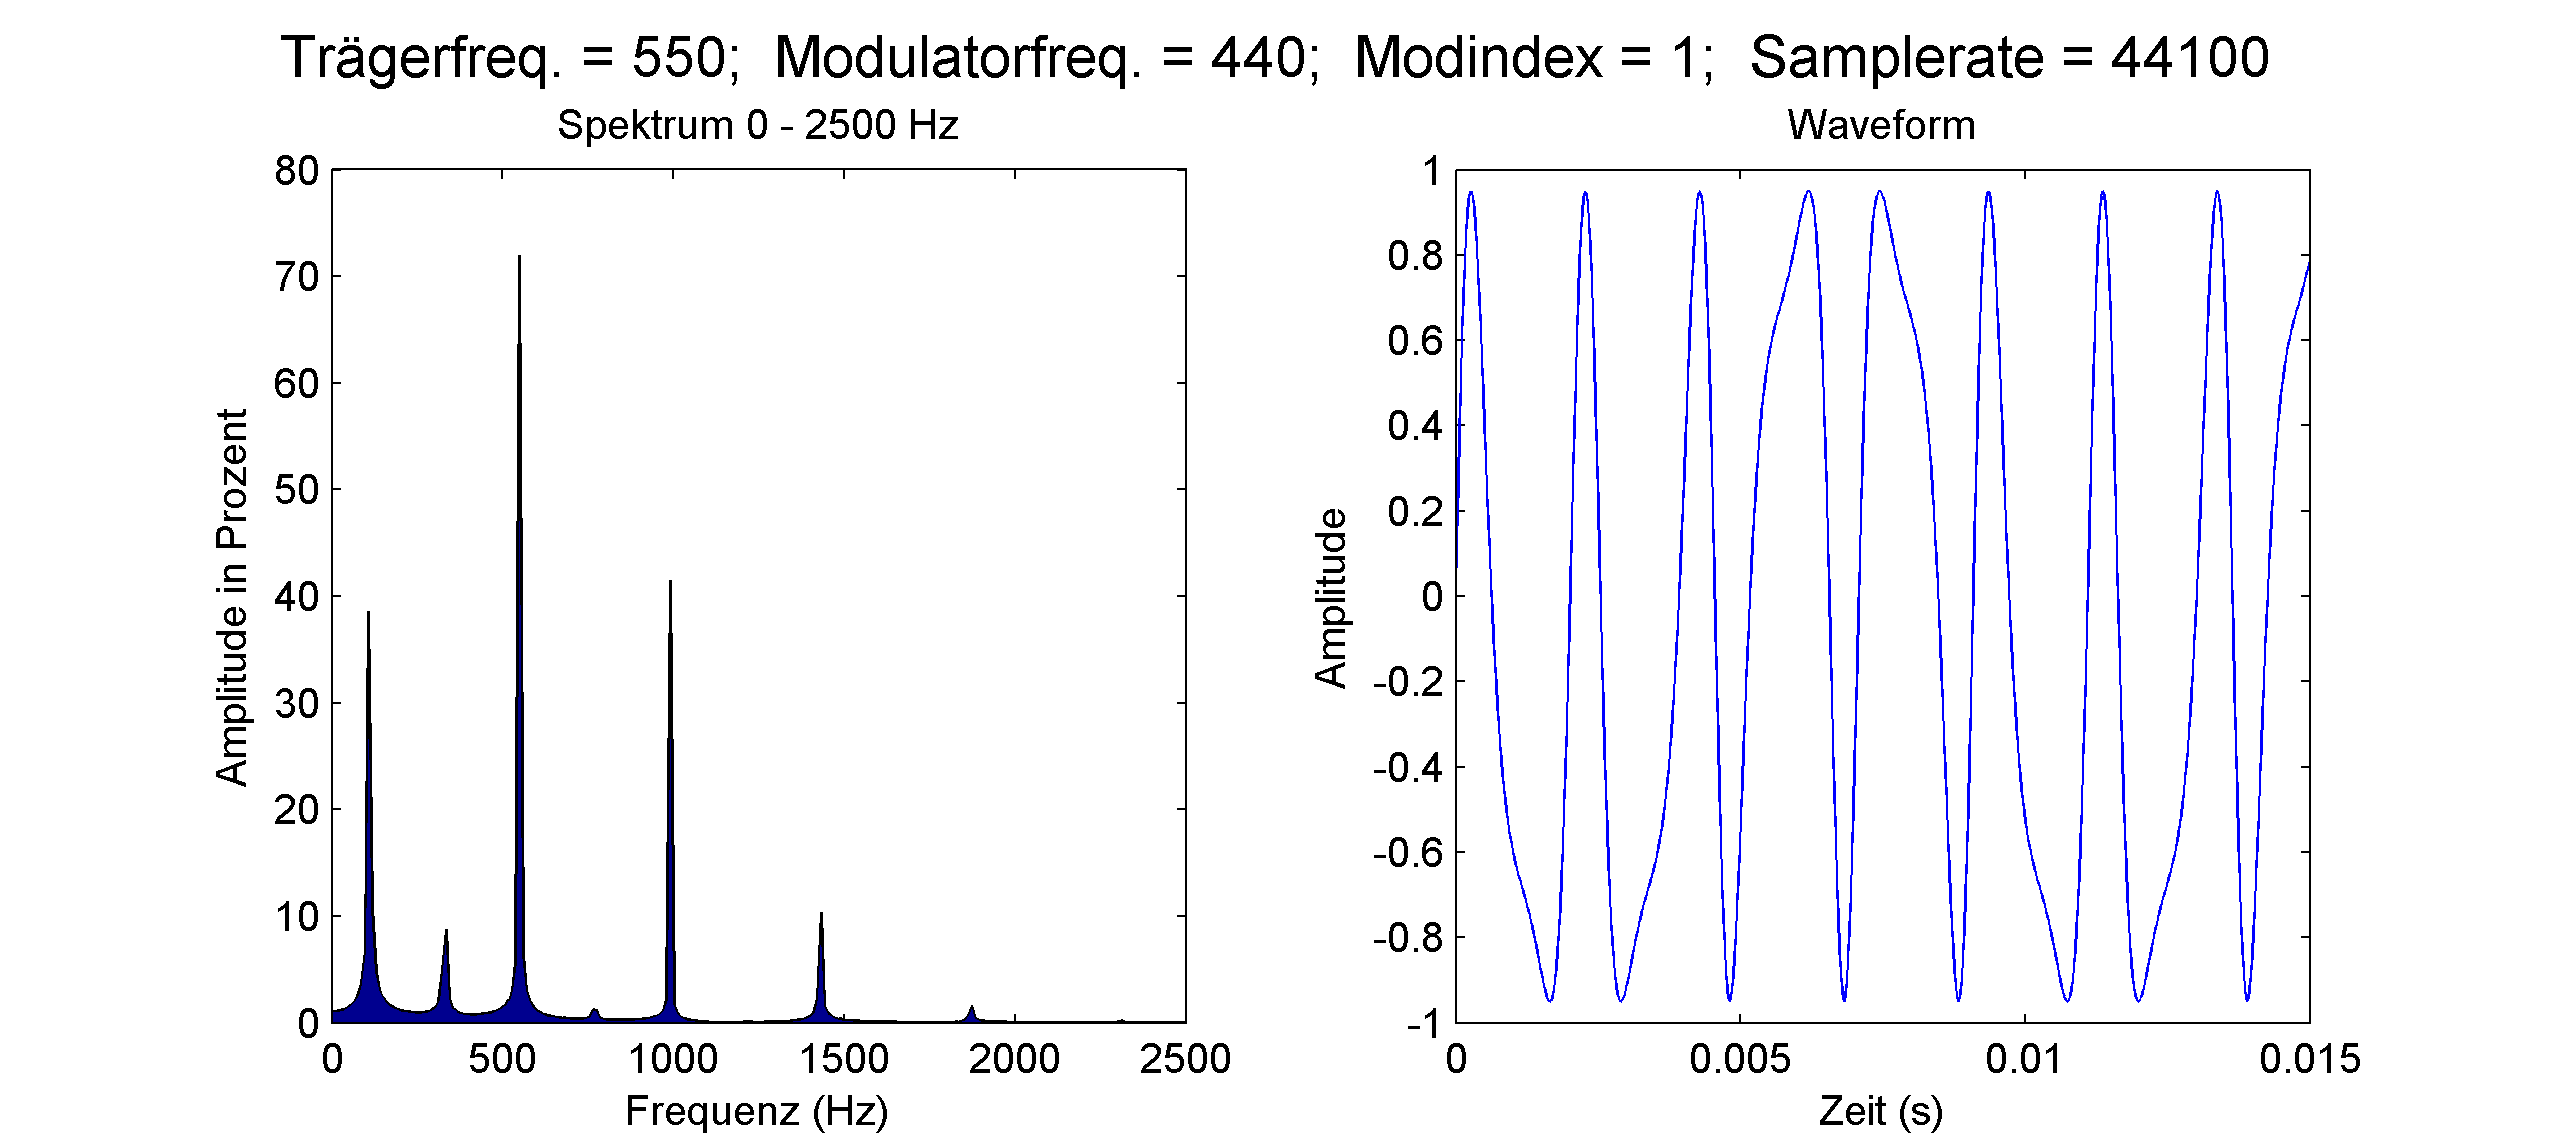
\includegraphics[width=0.95\textwidth]{parT2M.png}
\caption{Einfache FM mit $f_c = 550$, $w_m = 440$, $I = 1$. }
Quelle: Eigene Darstellung in MATLAB
\end{figure}
\FloatBarrier
Die parallele Modulation von T1 durch M1 sowie von T2 durch M2 wobei M1 und M2 exakt dieselben Einstellungen besitzen:
\FloatBarrier
\begin{figure} [ht]
\centering
  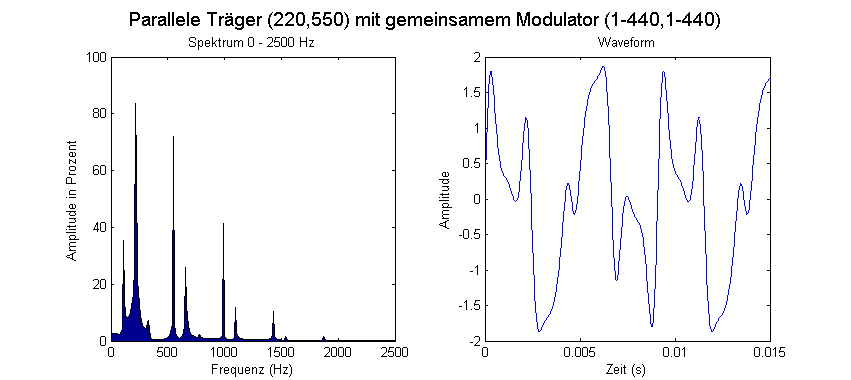
\includegraphics[width=0.95\textwidth]{parT1T2MM.png}
\caption{Parallele FM mit $f_{c1} = 220$, $f_{c2} = 550$, $w_{m1} = 440$, $w_{m2} = 440$, $I_1 = 1$, $I_2 = 1$. }
Quelle: Eigene Darstellung in MATLAB
\end{figure}
\FloatBarrier
Und abschließend zum Vergleich Wellenform und Frequenzspektrum zweier Träger, die sich denselben Modulator teilen:
\FloatBarrier
\begin{figure} [ht]
\centering
  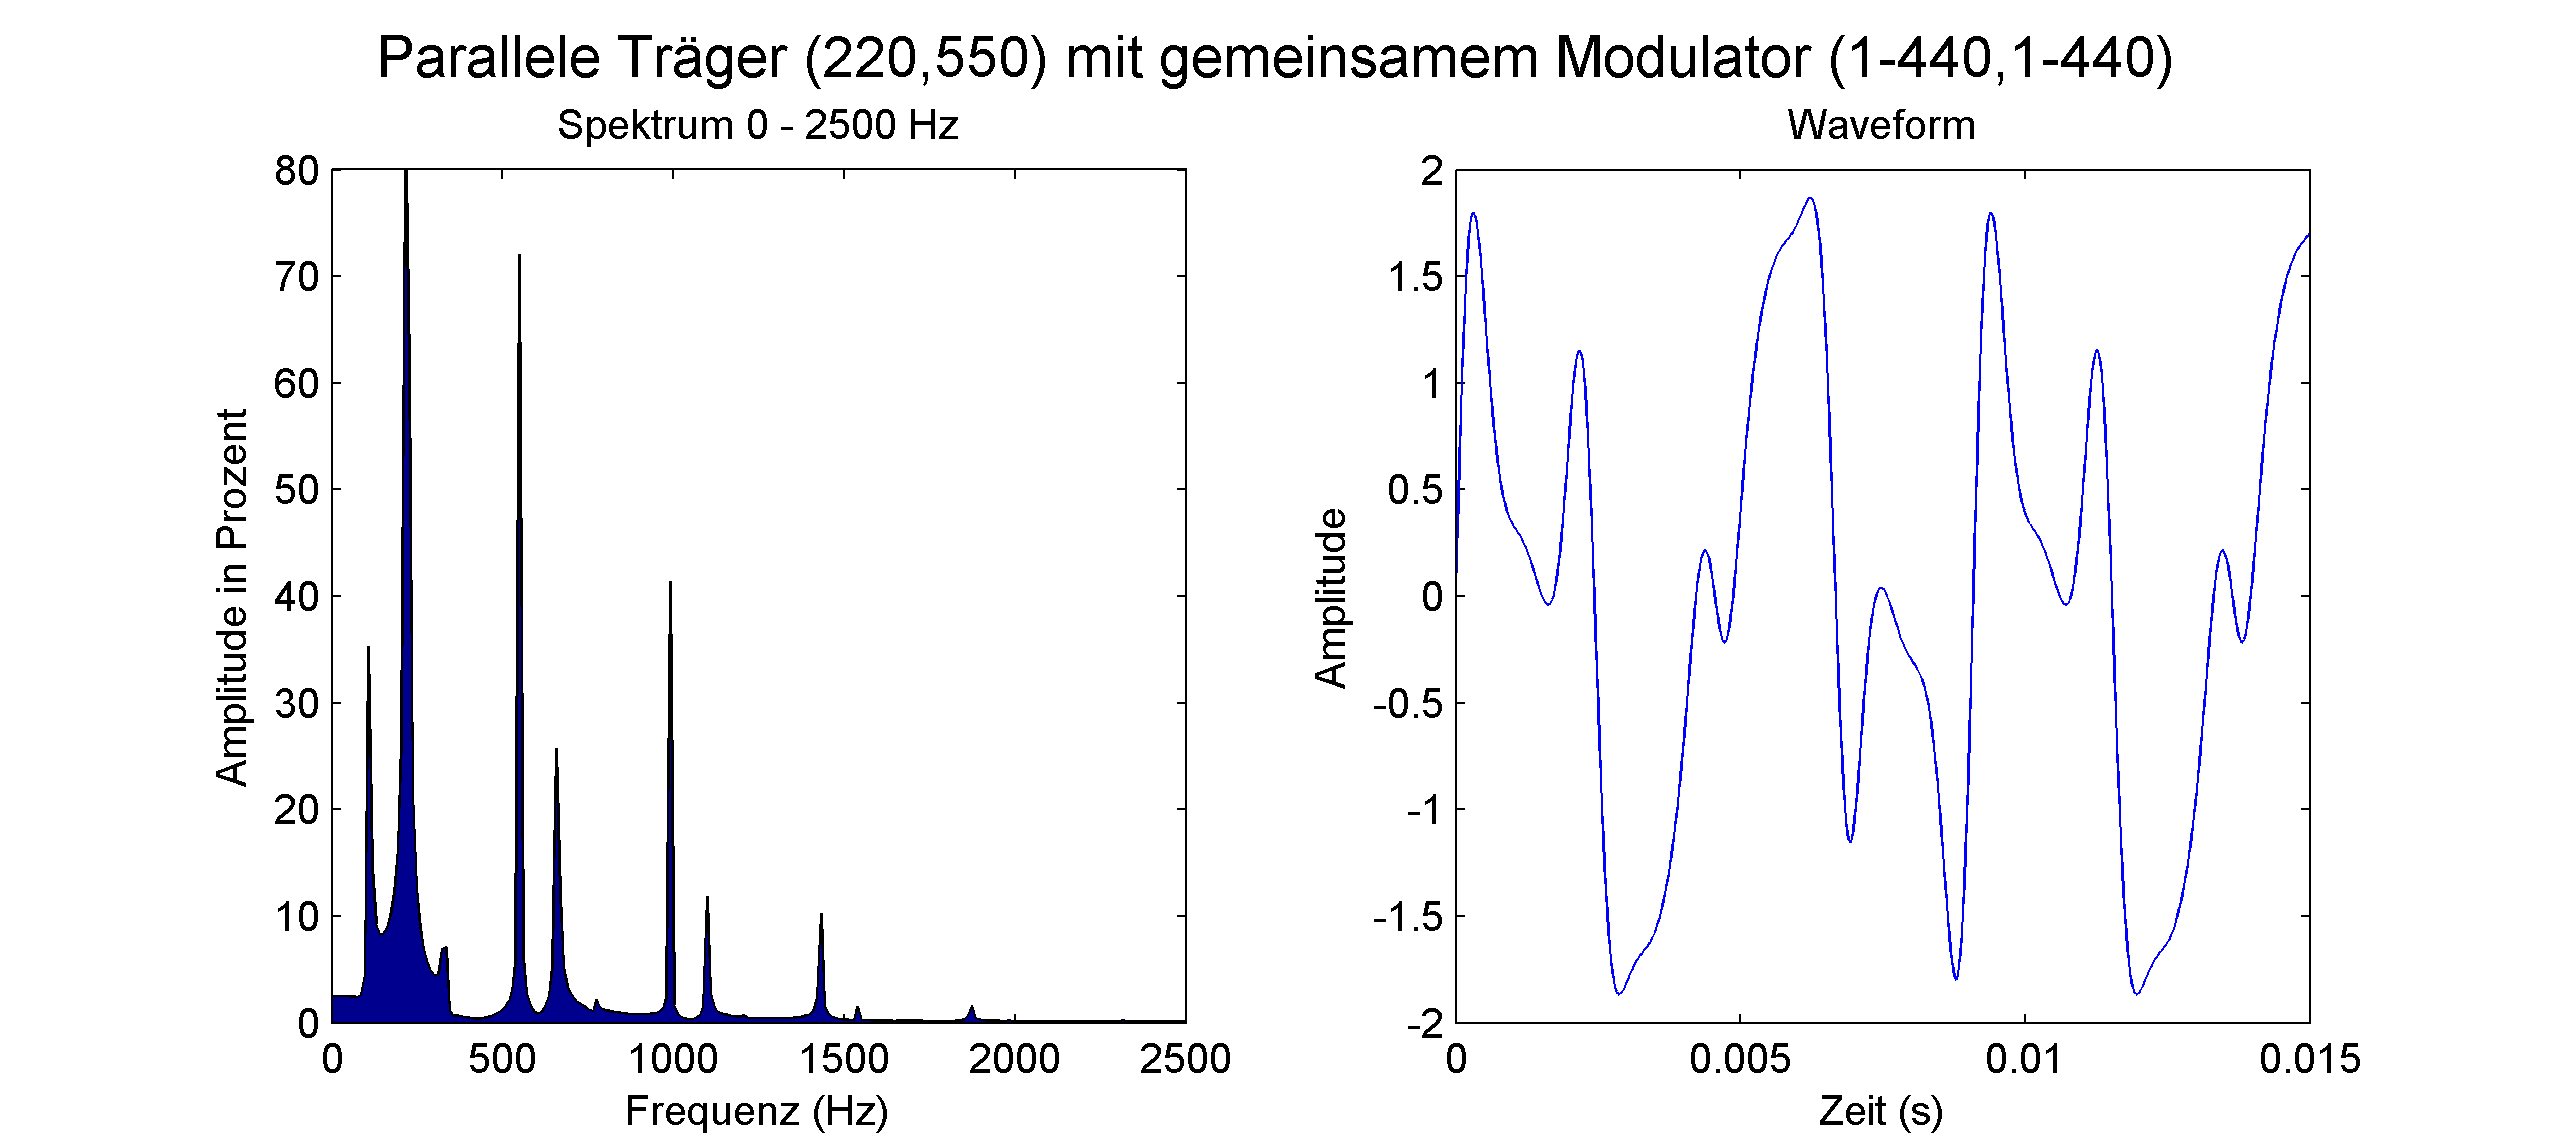
\includegraphics[width=0.95\textwidth]{parT1T2SameM.png}
\caption{Parallele FM mit $f_{c1} = 220$, $f_{c2} = 550$, $w_{m} = 440$, $I = 1$.  }
Quelle: Eigene Darstellung in MATLAB
\end{figure}
\FloatBarrier
Wie man sieht, sind die Spektren für die Modulation durch zwei verschiedene Modulatoren absolut identisch mit der Modulation durch denselben Modulator, sofern alle Modulatoren dieselben Einstellungen aufweisen.

\subsubsection{Einzelner Träger mit parallel geschaltetem Modulatorenpaar}
\label{singlecarryparallelmod}
Wird ein einzelner Träger $T$ von zwei parallel geschalteten Modulatoren $M1$ und $M2$ gleichzeitig moduliert, kann das erzeugte Frequenzspektrum nicht mehr einfach als Summe der Spektren zweier einfacher FM begriffen werden. Da sich die Auswirkungen der beiden Modulatoren auf den Träger gegenseitig beeinflussen, entstehen zahlreiche \textit{Kombinationsseitenfrequenzen} (\cite[S.117]{fmtheory})oder \textit{Intermodulationsfrequenzen]} (\cite{schottiWeb}). Das ist bereits aus der Funktion für diese Art der Parallelmodulation ersichtlich. Mit \cite[S.46]{schottstaedt} wird \ref{eq:SimpleFM} wie folgt um einen weiteren Modulator erweitert:
\begin{equation}
f_{FMparallel}(t) = \sin(w_ct + I_1\sin(w_{m1}t) + I\sin(w_{m2}t))
\end{equation}
Nach mehrmaliger Anwendung der trigonometrischen Additionstheoreme zeigt sich im Vergleich mit \ref{eq:BesselZwischenform} bereits, dass diese Formel eine Vielzahl zusätzlicher Terme generiert:
\begin{equation}
\begin{split}
\sin(w_ct + I_1\sin(w_{m1}t) + I\sin(w_{m2}t)) \\ &\quad = \sin(w_ct)\cos(I_1\sin(w_{m1}t))\cos(I\sin(w_{m2}t)) \\ &\quad + \cos(w_ct)\sin(I_1\sin(w_{m1}t))\cos(I\sin(w_{m2}t)) \\ &\quad +\cos(w_ct)\cos(I_1\sin(w_{m1}t))\sin(I\sin(w_{m2}t)) \\ &\quad -\sin(w_ct)\sin(I_1\sin(w_{m1}t))\sin(I\sin(w_{m2}t))
\end{split}
\end{equation}
Substituiert man auch hier wieder jedes \begin{math} \sin(I\sin(w_{mx}t) \end{math} mit \ref{eq:Besselsin} und \begin{math} \cos(I\sin(w_{mx}t)) \end{math}) mit \ref{eq:Besselcos} und wendet erneut die trigonometrischen Additionstheoreme an, so ergibt sich übersichtlich:
\begin{equation}\label{eq:ParallelKompakt}
\sin(w_ct + I_1\sin(w_{m1}t) + I\sin(w_{m2}t)) = \sum_{i=-\infty}^{\infty}\sum_{k=-\infty}^{\infty}J_i(I_1)J_k(I_2)\sin(w_ct + iw_{m1}t + kw_{m2}t)
\end{equation}
Damit ergeben sich exakt $i \times k$ Kombinationen der Besselfunktionskoeffizienten. Das bedeutet, dass bereits für alle Kombinationen der Indizes von -2 bis +2 ganze 25 verschiedene Terme generiert werden: 16 für die Kombinationsmöglichkeiten von 1 und 2 jeweils mit positivem oder negativem Vorzeichen; weitere 9 für die Kombinationen von 0 mit 1 oder 2 inklusive beider Vorzeichen; schließlich noch die einzelne Kombination von 0 mit sich selbst. Nachdem jeder Term für ein Seitenband steht, kann man sich die Komplexität des resultierenden Spektrums leicht ausmalen. Die entsprechenden Additionsterme lauten wie folgt:
\begin{equation}\label{eq:wallofequations}
\begin{split}
\sin&(w_ct + I_1\sin(w_{m1}t) + I\sin(w_{m2}t)) \\
&= J_0(I_1)J_0(I_2)\sin(w_ct) \\
&+ J_0(I_1)J_1(I_2)\sin(w_ct + w_{m2}t) - J_0(I_1)J_1(I_2)\sin(w_ct - w_{m2}t) \\
&+ J_0(I_1)J_2(I_2)\sin(w_ct + 2w_{m2}t) + J_0(I_1)J_1(I_2)\sin(w_ct - 2w_{m2}t) \\
&+ J_1(I_1)J_0(I_2)\sin(w_ct + w_{m1}t) - J_1(I_1)J_0(I_2)\sin(w_ct - w_{m1}t) \\
&+ J_1(I_1)J_1(I_2)\sin(w_ct + w_{m1}t + w_{m2}t) - J_1(I_1)J_1(I_2)\sin(w_ct + w_{m1}t - w_{m2}t) \\
&- J_1(I_1)J_1(I_2)\sin(w_ct - w_{m1}t + w_{m2}t) + J_1(I_1)J_1(I_2)\sin(w_ct - w_{m1}t - w_{m2}t) \\
&+ J_1(I_1)J_2(I_2)\sin(w_ct + w_{m1}t + 2w_{m2}t) + J_1(I_1)J_2(I_2)\sin(w_ct + w_{m1}t - 2w_{m2}t) \\
&- J_1(I_1)J_2(I_2)\sin(w_ct - w_{m1}t + 2w_{m2}t) - J_1(I_1)J_2(I_2)\sin(w_ct - w_{m1}t - 2w_{m2}t) \\
&+ J_2(I_1)J_0(I_2)\sin(w_ct + 2w_{m1}t) + J_2(I_1)J_0(I_2)\sin(w_ct - 2w_{m1}t) \\
&+ J_2(I_1)J_1(I_2)\sin(w_ct + 2w_{m1}t + w_{m2}t) + J_2(I_1)J_1(I_2)\sin(w_ct + 2w_{m1}t - w_{m2}t) \\
&+ J_2(I_1)J_1(I_2)\sin(w_ct - 2w_{m1}t + w_{m2}t) - J_2(I_1)J_1(I_2)\sin(w_ct - 2w_{m1}t - w_{m2}t) \\
&+ J_2(I_1)J_2(I_2)\sin(2w_ct + 2w_{m1}t + 2w_{m2}t) + J_2(I_1)J_2(I_2)\sin(2w_ct + 2w_{m1}t - 2w_{m2}t) \\
&+ J_2(I_1)J_2(I_2)\sin(2w_ct - 2w_{m1}t + 2w_{m2}t) + J_2(I_1)J_2(I_2)\sin(2w_ct - 2w_{m1}t - 2w_{m2}t) \\
&+ ... 
\end{split}
\end{equation}
Sofern zwei Zeilen eine Kombination von Besselkoeffizienten derselben zwei Ordnungen aufweisen, steht die ober Zeile für das obere Seitenfrequenzband, die Zeile darunter für das untere Seitenfrequenzband - zumindest sofern die Modulationsfrequenz von M1 größer ist, als jene von M2, sonst stehen die linken Terme beider Zeilen für das obere Frequenzband und die rechten Terme für das untere. Die Lage eines Frequenzbands ergibt sich also stets durch den Abstand eines Vielfachen der ersten Modulatorfrequenz vom Träger nach beiden Seiten, und um diesen Punkt herum dann jeweils um ein Vielfaches der zweiten Modulatorfrequenz nach beiden Seiten versetzt. Die Amplitude des jeweiligen Bandes liefert das Produkt der Besselkoeffizienten. 

Eine Abkürzung, um auf die Additionsterme für das Spektrum oben zu gelangen, sei hier noch kurz präsentiert: Sieht man sich z.B. die beiden Zeilen mit den Besselkoeffizienten \begin{math} J_1J_2 \end{math} an, so kann man sich klarmachen, dass diese beiden Zeilen zusammen die Kombinationen der Ordnungen (1,2),(1,-2),(-1,2),(-1,-2) abdecken (sprich, die Wechselwirkung zwischen erstem und zweitem Frequenzband). Nun weiß man bereits, dass man 4 Terme braucht. Innerhalb jedes einzelnen Terms bekommt jeweils \begin{math} w_{m1} \end{math} als Koeffizient die erste Vektorkomponente, \begin{math} w_{m2} \end{math} die zweite Vektorkomponente. Für den Vektor (1,-2) lautet der Term somit \begin{math} J_1(I_1)J_2(I_2)\sin(w_ct + w_{m1}t - 2w_{m2}t) \end{math}. Der gesamte Term erhält als Vorzeichen noch das Produkt der Vorzeichen der Vektorkomponenten, jeweils potenziert mit dem Betrag der jeweiligen Komponente. Für das gewählte Beispiel wäre das folglich \begin{math} (1)^1*(-1)^2 = 1 \end{math} - der Term bekommt also ein positives Vorzeichen. Die Bedingung des Potenzierens der Vorzeichen leitet sich dabei aus folgender Eigenschaft der Besselfunktion (\cite[S.358, Satz~9.1.5]{abramowitz}) ab:
\begin{equation}
J_{-n}(x) = (-1)^nJ_n(x)
\end{equation}
Um die Zusammenhänge grafisch zu veranschaulichen, nehmen wir zunächst einen Träger und modulieren ihn durch $M1$. Um den Effekt von Reflektionen an der 0Hz-Barriere durch negative Frequenzen zu verringern, setzen wir diesmal die Trägerfrequenz auf $1250Hz$. 
\FloatBarrier
\begin{figure} [ht]
\centering
  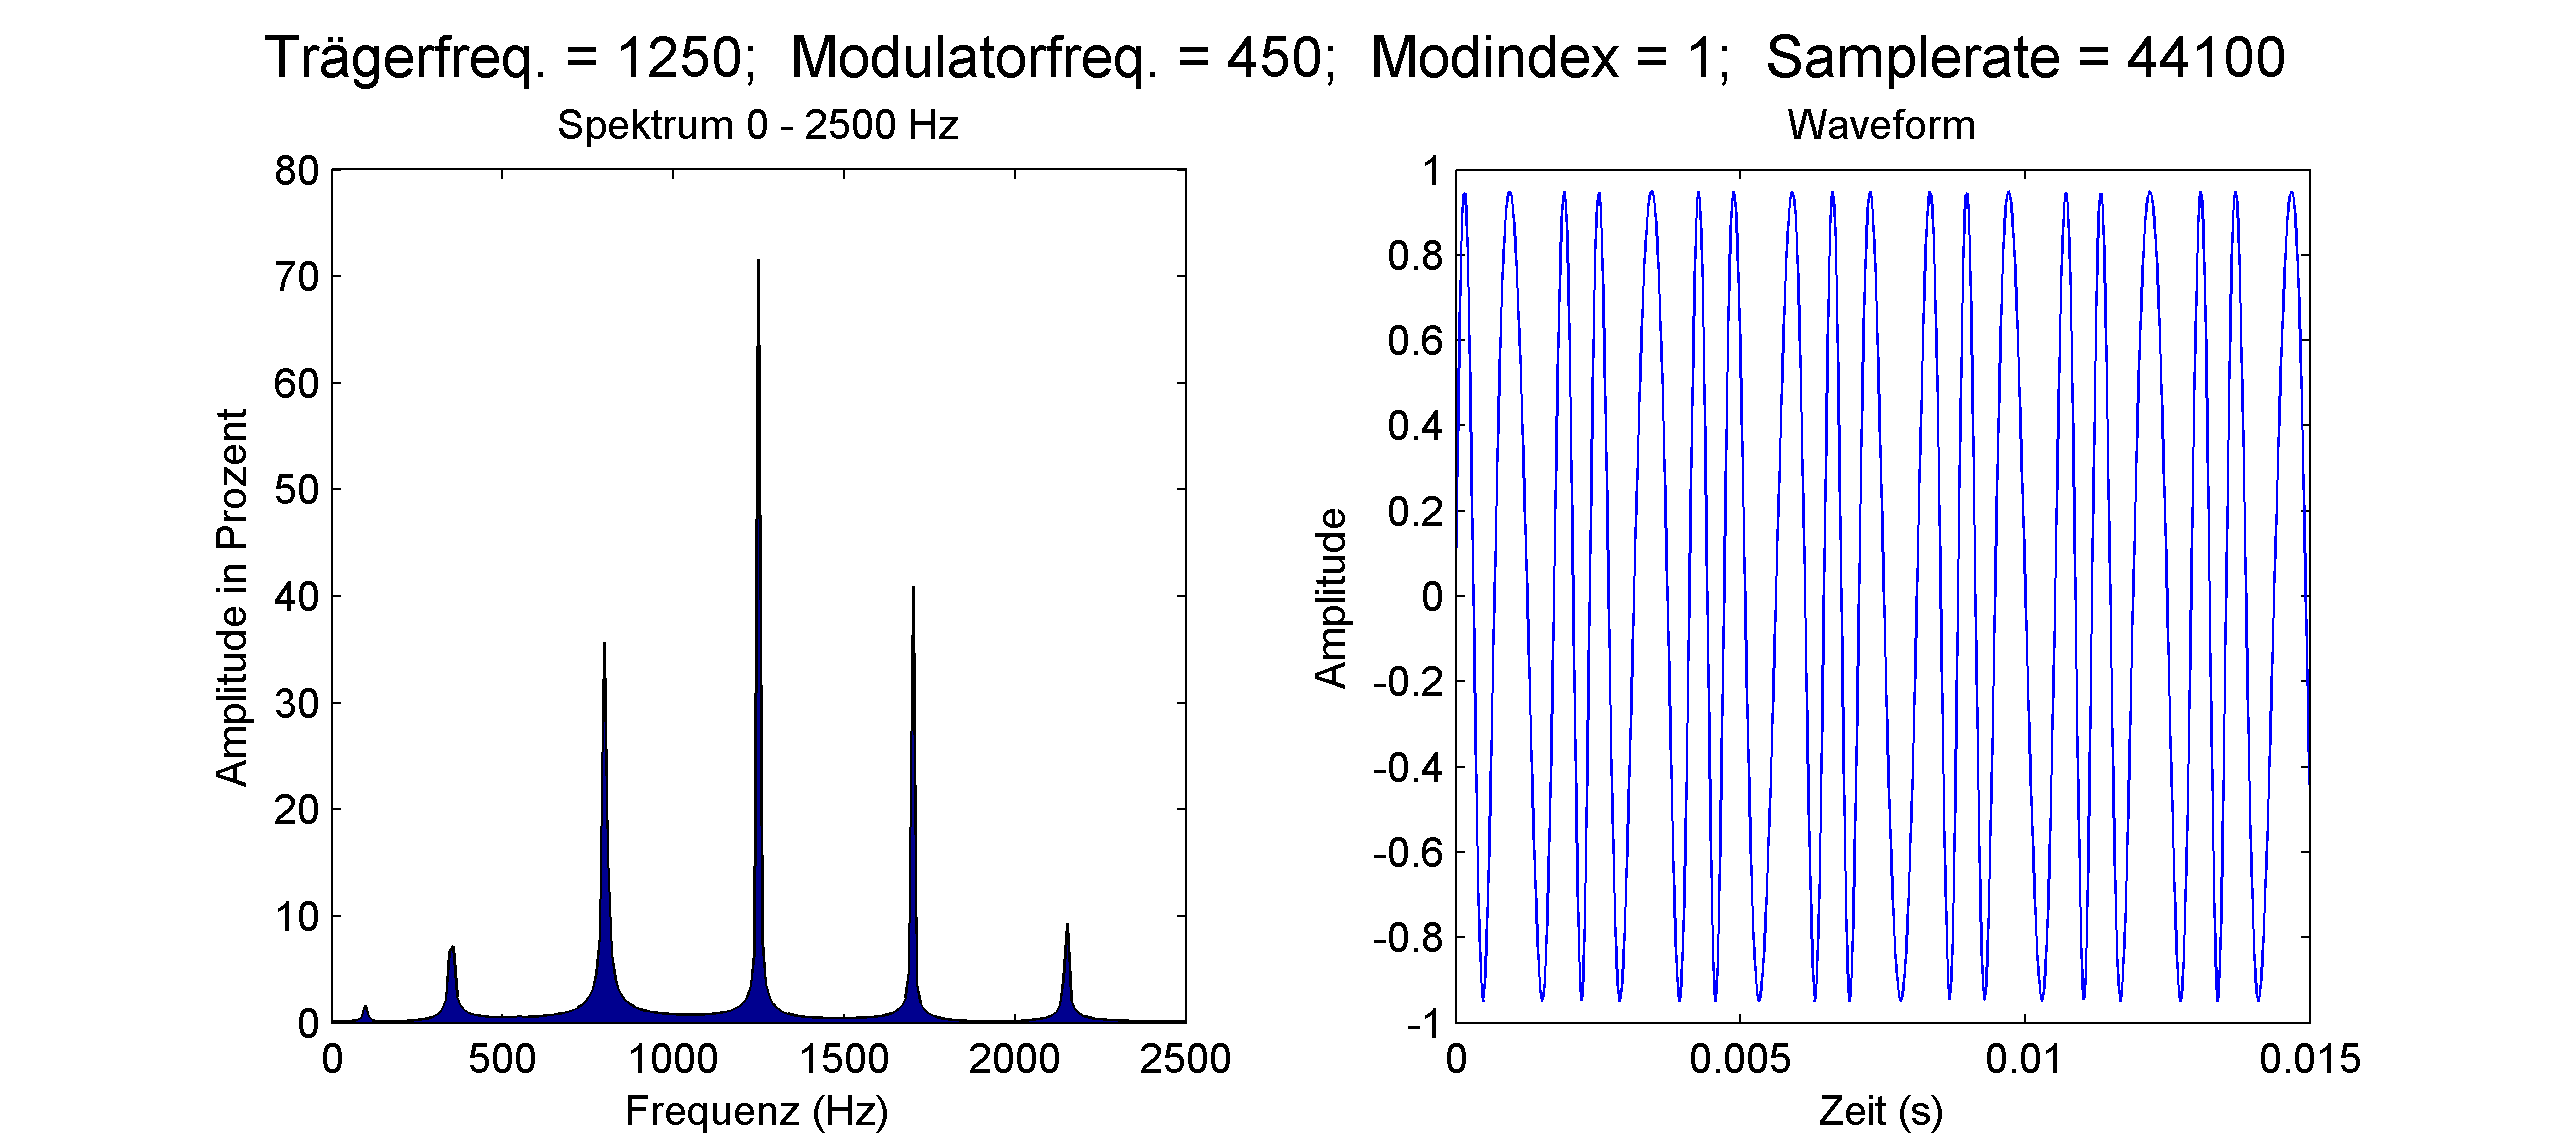
\includegraphics[width=0.95\textwidth]{parTM.png}
\caption{Einfache FM mit $f_c = 1250$, $w_m = 450$, $I = 1$. }
Quelle: Eigene Darstellung in MATLAB
\end{figure}
\FloatBarrier
Man sieht im Spektrum, dass wie erwartet die Trägerfrequenz bei 1250Hz liegt, und das erste Seitenband bei $ 1250 + 450 =$ 1700Hz. Die Additionsterme aus Gleichung \ref{eq:wallofequations} legen nun nahe, dass bei einer Modulation eines Trägers durch zwei parallele Modulatoren jeweils oberhalb und unterhalb jedes von $M1$ erzeugten Seitenbandes in Abständen der Frequenz von $M2$ dessen Seitenbänder liegen sollten. Zum Vergleich betrachten wir also zuerst noch einen Träger mit einer Frequenz, die dem ersten Seitenband von eben, 1700Hz, entspricht, und modulieren diesen durch $M2 =$ 180Hz, da wir so eine Prognose für die Seitenbänder von $M2$ bei einer gemeinsamen Modulation des Trägers erhalten. Beide Modulationsindizes erhalten den Wert 1, da die Besselfunktionen mit steigender Ordnung für dieses Argument kontinuierlich kleiner werden. Damit werden die Frequenzbänder niedriger Ordnung stets erkennbarer sein als ihre Nachbarn höherer Ordnung, und der Vergleich der beiden gewählten Einzelmodulationen mit der Parallelmodulation gewinnt an Aussagekraft.
\FloatBarrier
\begin{figure} [ht]
\label{par1}
\centering
  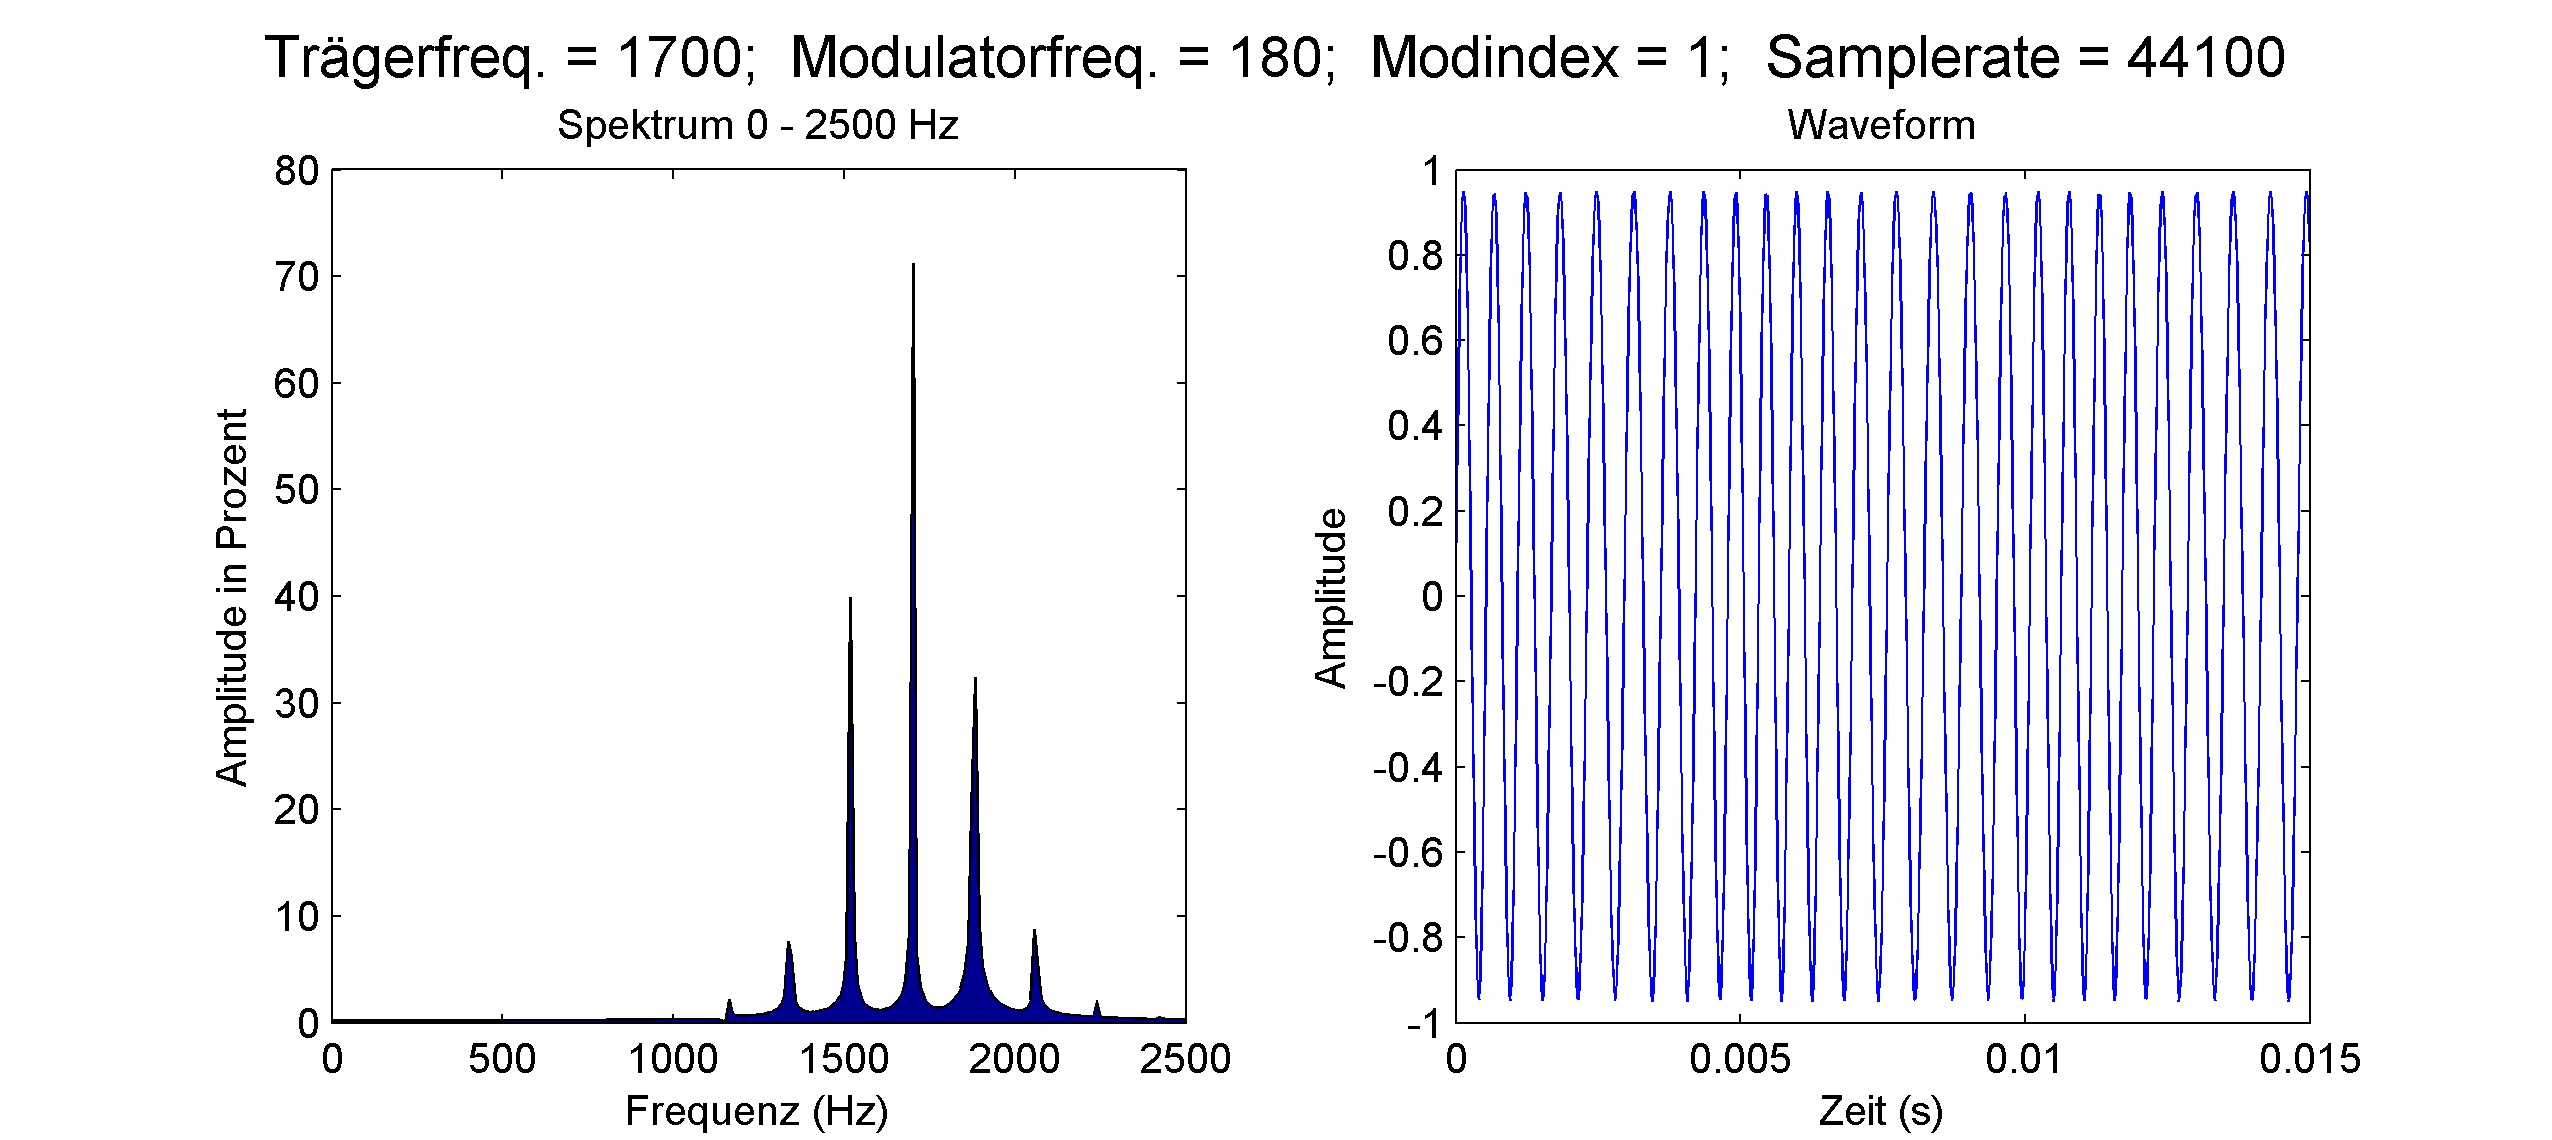
\includegraphics[width=0.95\textwidth]{par2TM.png}
\caption{Einfache FM mit $f_c = 1700$, $w_m = 180$, $I = 1$. }
Quelle: Eigene Darstellung in MATLAB
\end{figure}
\FloatBarrier
Hier nun die Anwendung beider Modulatoren mit unveränderten Einstellungen auf den Träger des ersten Spektrums mit einer Trägerfrequenz von 1250Hz. Es steht zu erwarten, dass der erste Modulator Seitenbänder bei 800Hz und 1700Hz erzeugt, der zweite von dort ausgehend jeweils oberhalb und unterhalb eines im Abstand von 180Hz. Die beiden Spektren oben sollten sich so ungefähr im folgenden gemeinsamen Spektrum wiederfinden lassen, zuzüglich Frequenzbändern von 180Hz oberhalb und unterhalb von 1250Hz:
\FloatBarrier
\begin{figure} [ht]
\centering
  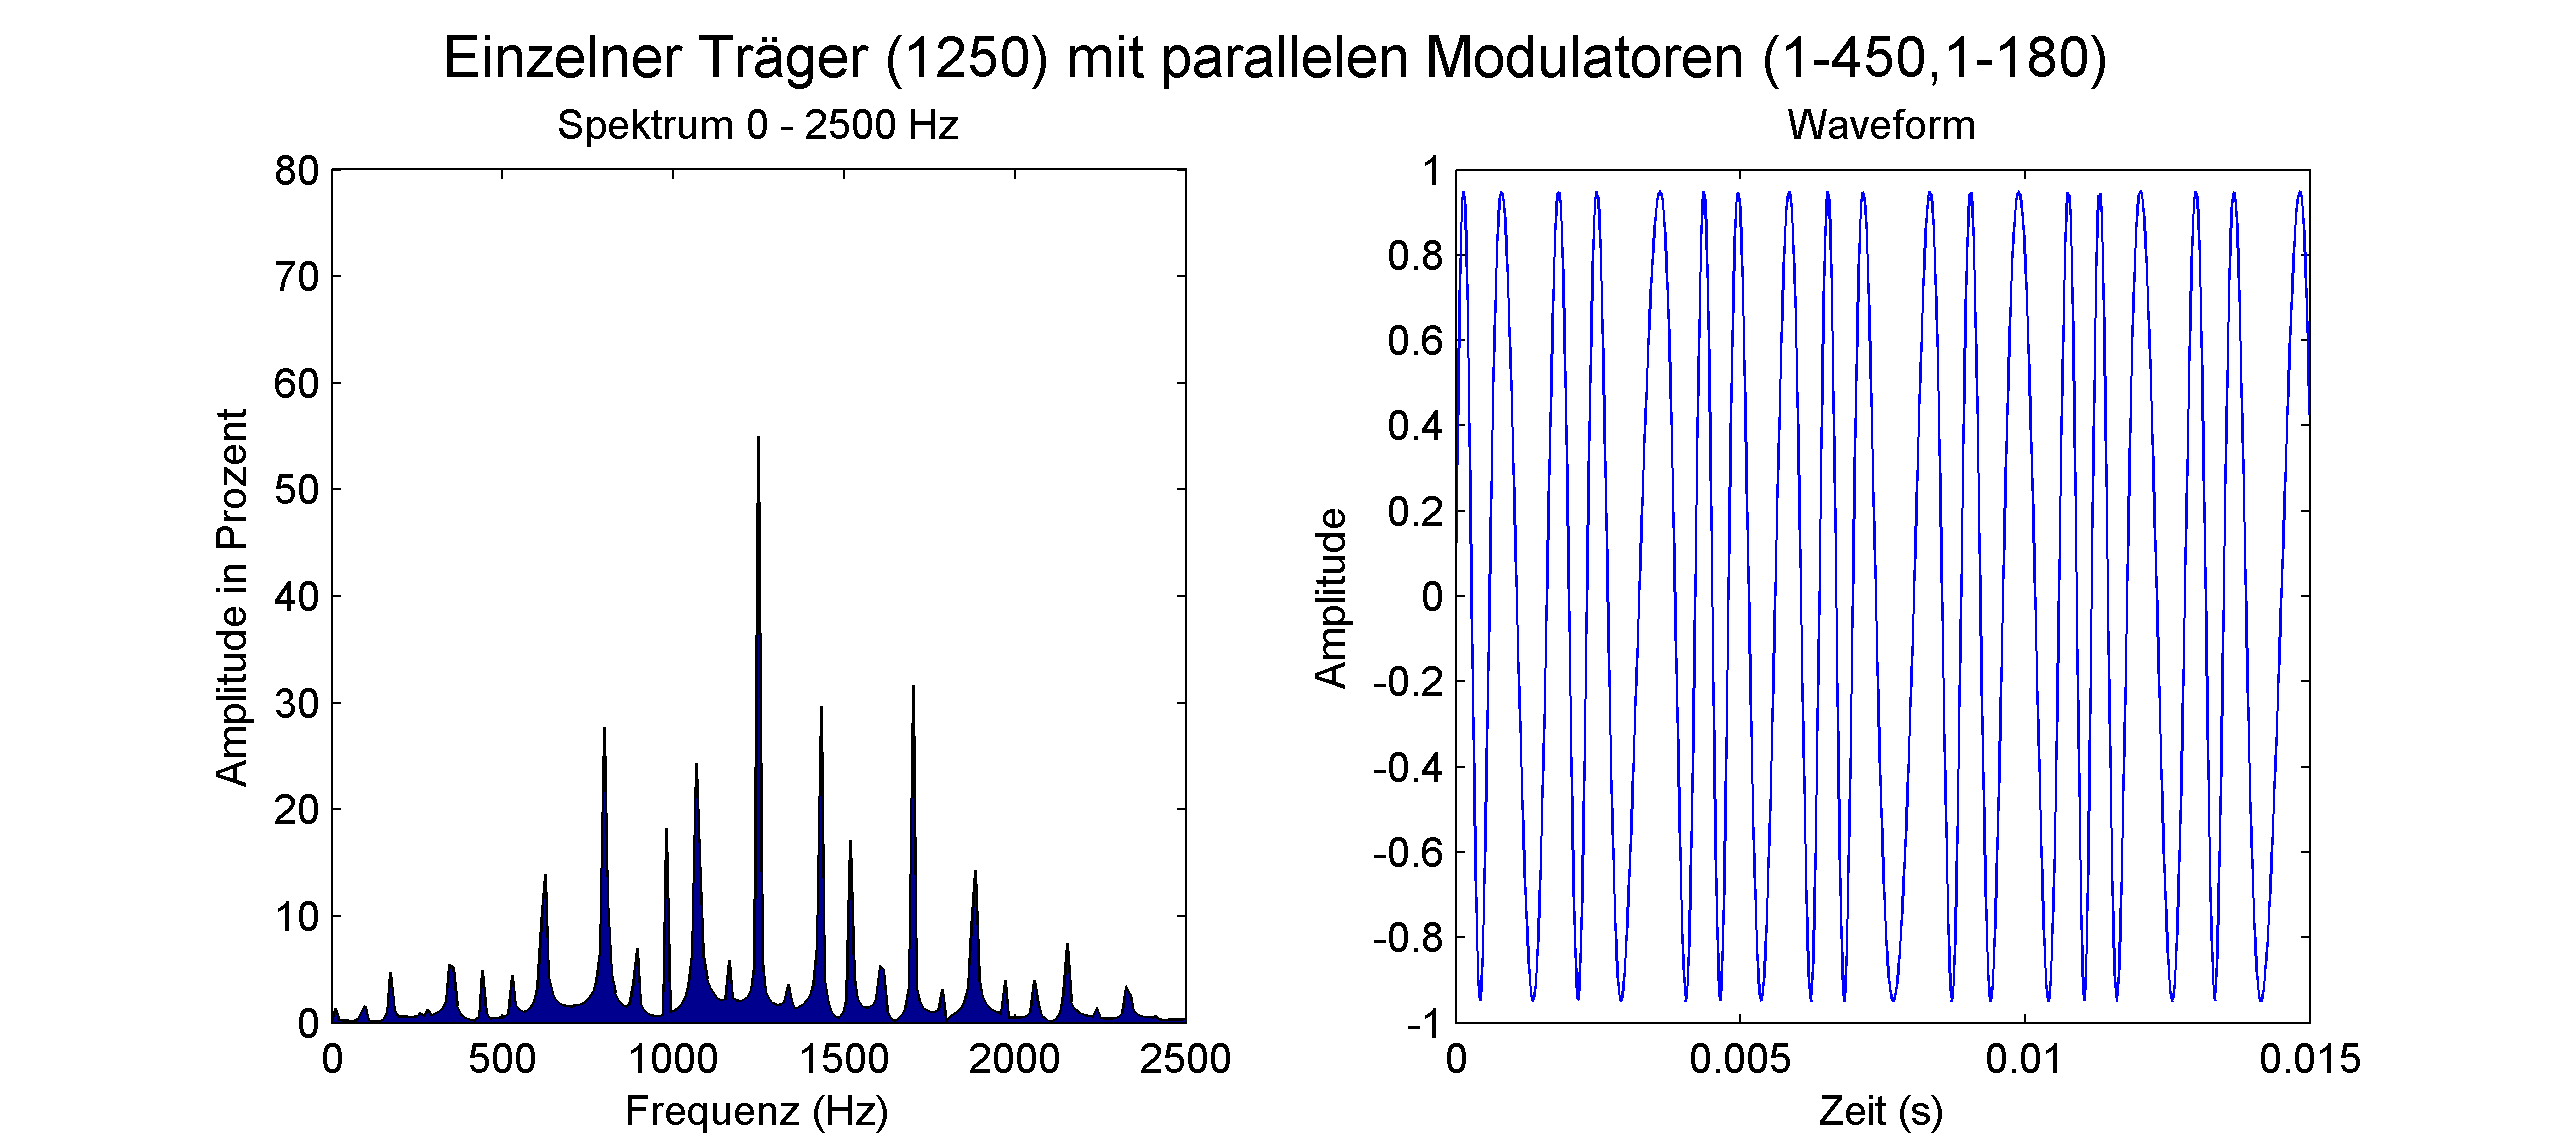
\includegraphics[width=0.95\textwidth]{parTM1M2.png}
\caption{Parallele FM mit $f_c = 1250$, $w_{m1} = 450$, $w_{m2} = 180$, $I_1 = 1$, $I_2 = 1$. }
Quelle: Eigene Darstellung in MATLAB
\end{figure}
\FloatBarrier
Die Prognose bestätigt sich: Betrachtet man den Bereich um 1700Hz, so findet man dort das Spektrum von \ref{par1}. Auch die Seitenbänder im Abstand von 180Hz um den Träger sind klar zu erkennen.

\subsection{Kaskadenschaltung: Einzelträger mit Modulatorenpaar in Reihe}
\label{cascade}

Den bisher betrachteten Schaltungen war gemein, dass unabhängig davon, ob ein Träger, mehrere Träger, ein Modulator oder mehrere Modulatoren verwendet worden sind, in keinem der Fälle ein Modulator selbst durch einen weiteren Modulator moduliert worden ist. Diese Kombinationsmöglichkeit eines Trägers sowie zweier Modulatoren stellt jedoch ein weiteres mächtiges Instrument der FM dar und soll im Folgenden beschrieben werden. 

Die Modulation eines Trägers durch einen Modulator, der selbst wiederum durch einen weiteren Modulator moduliert wird, also die Reihenschaltung $T<M1<M2$, lässt sich in die bisher gewählte Formel für die einfache FM,
\begin{equation}\label{eq:fmsimplex}
f_{FM}(t) = \sin(w_ct + I\sin(w_mt))
\end{equation}
wenig überraschend wie folgt integrieren (\cite[S.48]{schottstaedt}):
\begin{equation}\label{eq:fmkaskade}
f_{FMkaskade}(t) = \sin(w_ct + I_1\sin(w_{m1}t + I_2\sin(w_{m2}t)))
\end{equation}
Bereits an der Funktion lässt sich der verschachtelte Charakter der Kaskadenschaltung ablesen: Der Modulationswert $ I\sin(w_mt) $ wird durch den Wert einer weiteren, kompletten Frequenzmodulation $ I_2\sin(w_{m1}t + I_2\sin(w_{m2}t)) $ ersetzt. 

Für die Herleitung des Frequenzspektrums brauchen keine ausschweifenden Umformungen durch Additionstheoreme mehr vorgenommen oder Eigenschaften der Besselfunktion ausgenutzt werden: Hat man \ref{eq:fmsimplex}, \ref{eq:fmkaskade} sowie \ref{eq:freqfm} bereits bestimmt, so kann in der Formel für das Frequenzspektrum zu \ref{eq:fmsimplex}, also in
\begin{equation}\label{eq:freqfm}
\sin(w_ct + I\sin(w_mt)) = \sum_{n=-\infty}^{\infty}J_n(I)\sin(w_ct+nw_mt)
\end{equation}
einfach $ \sin(w_mt) $ durch $ \sin(w_{m1}t + I_2\sin(w_{m2}t)) $ ersetzt werden. Eine Reihe einfacher Umformungen führt dann zur Formel für das Frequenzsspektrum der Kaskadenschaltung:
\begin{equation}
\begin{split}
& \quad \sum_{n=-\infty}^{\infty}J_n(I_1)sin(w_{c}t + nI_2(sin(w_{m2}t))) \\
&= \sum_{n=-\infty}^{\infty}J_n(I_1)sin(w_{c}t+n(w_{m1}t + I_2(sin(w_{m2}t)))) \\
&= \sum_{n=-\infty}^{\infty}J_n(I_1)sin((w_{c}t+nw_{m1}t) + (I_2n(sin(w_{m2}t))))
\end{split}
\end{equation}
Da hier die beiden Klammern in der Sinusfunktion zusammen exakt einer eigenständigen FM entsprechen, kann das Argument für den Sinus auch durch die Formel zur Berechnung ihres Spektrums \ref{eq:freqfm} substituiert werden. Es ergibt sich damit für das Frequenzspektrum der Kaskadenschaltung wie in \cite{schottiWeb}:
\begin{equation}
\sum_{n=-\infty}^{\infty}\sum_{n=-\infty}^{\infty}J_n(I_1)J_n(\mathbf{n}I_2)sin(w_{c}t+nw_{m1}t + kw_{m2}t)
\end{equation}
Damit entspricht die Formel für das Frequenzspektrum der Kaskadenschaltung exakt jener für die Parallelschaltung \ref{eq:ParallelKompakt}, mit einem kleinen Zusatz: Es wird bei der Kaskadenschaltung zusätzlich der Modulationsindex $ I_2 $ des äußersten Modulators $M2$ mit der Ordnung $ n $ des ersten Besselkoeffizienten multipliziert und erst anschließend als Argument an die Besselfunktion gereicht. Damit ändern sich auch bei den Additionstermen für das Spektrum im Vergleich zur Parallelschaltung \ref{eq:wallofequations} lediglich die Koeffizienten:
\begin{equation}
\begin{split}
\sin&(w_ct + I_1\sin(w_{m1}t) + I\sin(w_{m2}t)) \\
&= J_0(I_1)J_0(\mathbf{0}I_2)\sin(w_ct) \\
&+ J_0(I_1)J_1(\mathbf{0}I_2)\sin(w_ct + w_{m2}t) - J_0(I_1)J_1(I_2)\sin(w_ct - w_{m2}t) \\
&+ J_0(I_1)J_2(\mathbf{0}I_2)\sin(w_ct + 2w_{m2}t) + J_0(I_1)J_1(I_2)\sin(w_ct - 2w_{m2}t) \\
&+ J_1(I_1)J_0(\mathbf{1}I_2)\sin(w_ct + w_{m1}t) - J_1(I_1)J_0(I_2)\sin(w_ct - w_{m1}t) \\
&+ J_1(I_1)J_1(\mathbf{1}I_2)\sin(w_ct + w_{m1}t + w_{m2}t) - J_1(I_1)J_1(I_2)\sin(w_ct + w_{m1}t - w_{m2}t) \\
&- J_1(I_1)J_1(\mathbf{1}I_2)\sin(w_ct - w_{m1}t + w_{m2}t) + J_1(I_1)J_1(I_2)\sin(w_ct - w_{m1}t - w_{m2}t) \\
&+ J_1(I_1)J_2(\mathbf{1}I_2)\sin(w_ct + w_{m1}t + 2w_{m2}t) + J_1(I_1)J_2(I_2)\sin(w_ct + w_{m1}t - 2w_{m2}t) \\
&- J_1(I_1)J_2(\mathbf{1}I_2)\sin(w_ct - w_{m1}t + 2w_{m2}t) - J_1(I_1)J_2(I_2)\sin(w_ct - w_{m1}t - 2w_{m2}t) \\
&+ J_2(I_1)J_0(\mathbf{2}I_2)\sin(w_ct + 2w_{m1}t) + J_2(I_1)J_0(I_2)\sin(w_ct - 2w_{m1}t) \\
&+ J_2(I_1)J_1(\mathbf{2}I_2)\sin(w_ct + 2w_{m1}t + w_{m2}t) + J_2(I_1)J_1(I_2)\sin(w_ct + 2w_{m1}t - w_{m2}t) \\
&+ J_2(I_1)J_1(\mathbf{2}I_2)\sin(w_ct - 2w_{m1}t + w_{m2}t) - J_2(I_1)J_1(I_2)\sin(w_ct - 2w_{m1}t - w_{m2}t) \\
&+ J_2(I_1)J_2(\mathbf{2}I_2)\sin(2w_ct + 2w_{m1}t + 2w_{m2}t) + J_2(I_1)J_2(I_2)\sin(2w_ct + 2w_{m1}t - 2w_{m2}t) \\
&+ J_2(I_1)J_2(\mathbf{2}I_2)\sin(2w_ct - 2w_{m1}t + 2w_{m2}t) + J_2(I_1)J_2(I_2)\sin(2w_ct - 2w_{m1}t - 2w_{m2}t) \\
&+ ... 
\end{split}
\end{equation}
\label{Kaskadenspecials}
Man sieht sofort, dass damit erstens die Trägerfrequenz ausschließlich durch $ I_1 $ definiert wird, da $ I_2 $ bei der Trägerfrequenz mit $0$ multipliziert wird und die Besselfunktion der nullten Ordnung für das Argument $0$ genau den Wert $1$ zurückgibt. Zweitens muss sich für höhere Seitenbänder der Modulationsindex für $M2$, also $ I_2 $, und damit auch die Gesamtheit der Kombinationsseitenfrequenzen höherer Ordnung im Vergleich zur Parallelmodulation stärker auf das resultierende Spektrum auswirken, da $ I_2 $ dort ja mit größeren $n$ multipliziert wird. Drittens entfallen alle Kombinationsseitenfrequenzen mit dem Besselkoeffizienten der Ordnung $0$ des inneren Modulators vollständig, da die dadurch bedingte Multiplikation mit $n = 0$ im Argument für die Besselfunktionen mit Ordnung $>0$ des äußeren Modulators immer den Wert $0$ zurückliefern (siehe \ref{fig:bessel2D}). 

Visualisiert in MATLAB zeigt sich, dass sich erwartungsgemäß um jedes Seitenband von $T$ und $M1$ die Seitenbänder von $M1$ und $M2$ ausbreiten. Mit denselben Einstellungen wie in \ref{singlecarryparallelmod} sieht das Spektrum von $T$ moduliert durch $M1$ natürlich immer noch genauso aus:
\FloatBarrier
\begin{figure} [ht]
\centering
  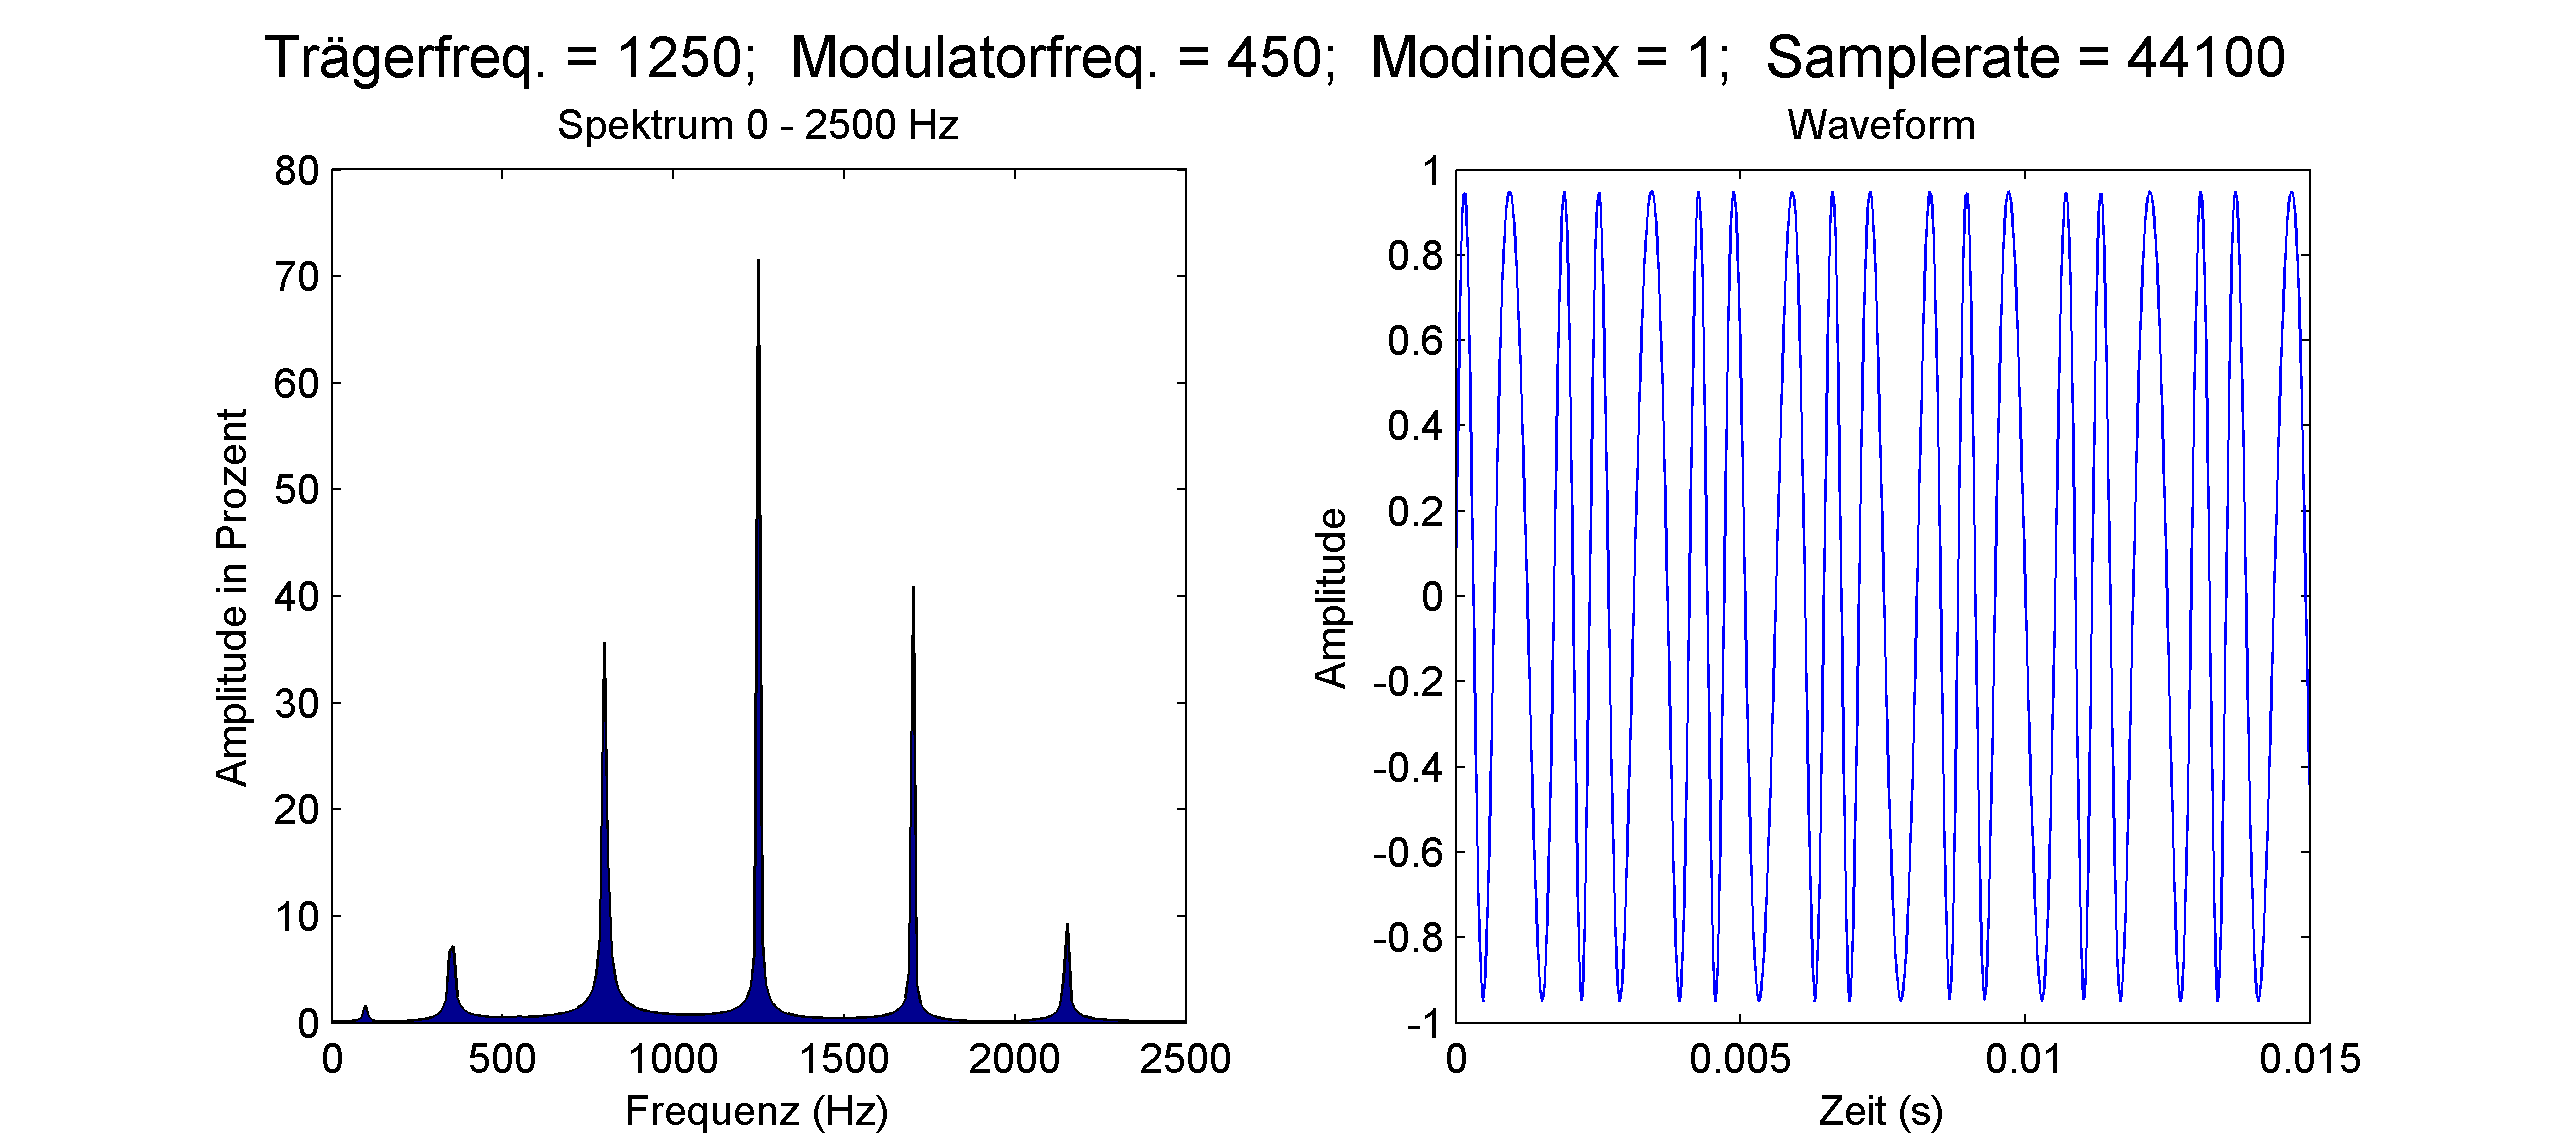
\includegraphics[width=0.95\textwidth]{parTM.png}
\caption{Einfache FM mit $f_c = 1250$, $w_m = 450$, $I = 1$. }
Quelle: Eigene Darstellung in MATLAB
\end{figure}
\FloatBarrier
Nun das Spektrum von $T$ nach der Modulation durch $M1$, moduliert durch $M2$. Zum Nachstellen wurde ein Träger mit 1700Hz moduliert, da dort das erste Seitenband aus obiger Modulation landet, und durch einen Modulator mit den Einstellungen von $M2$ moduliert:
\FloatBarrier
\begin{figure} [ht]
\centering
  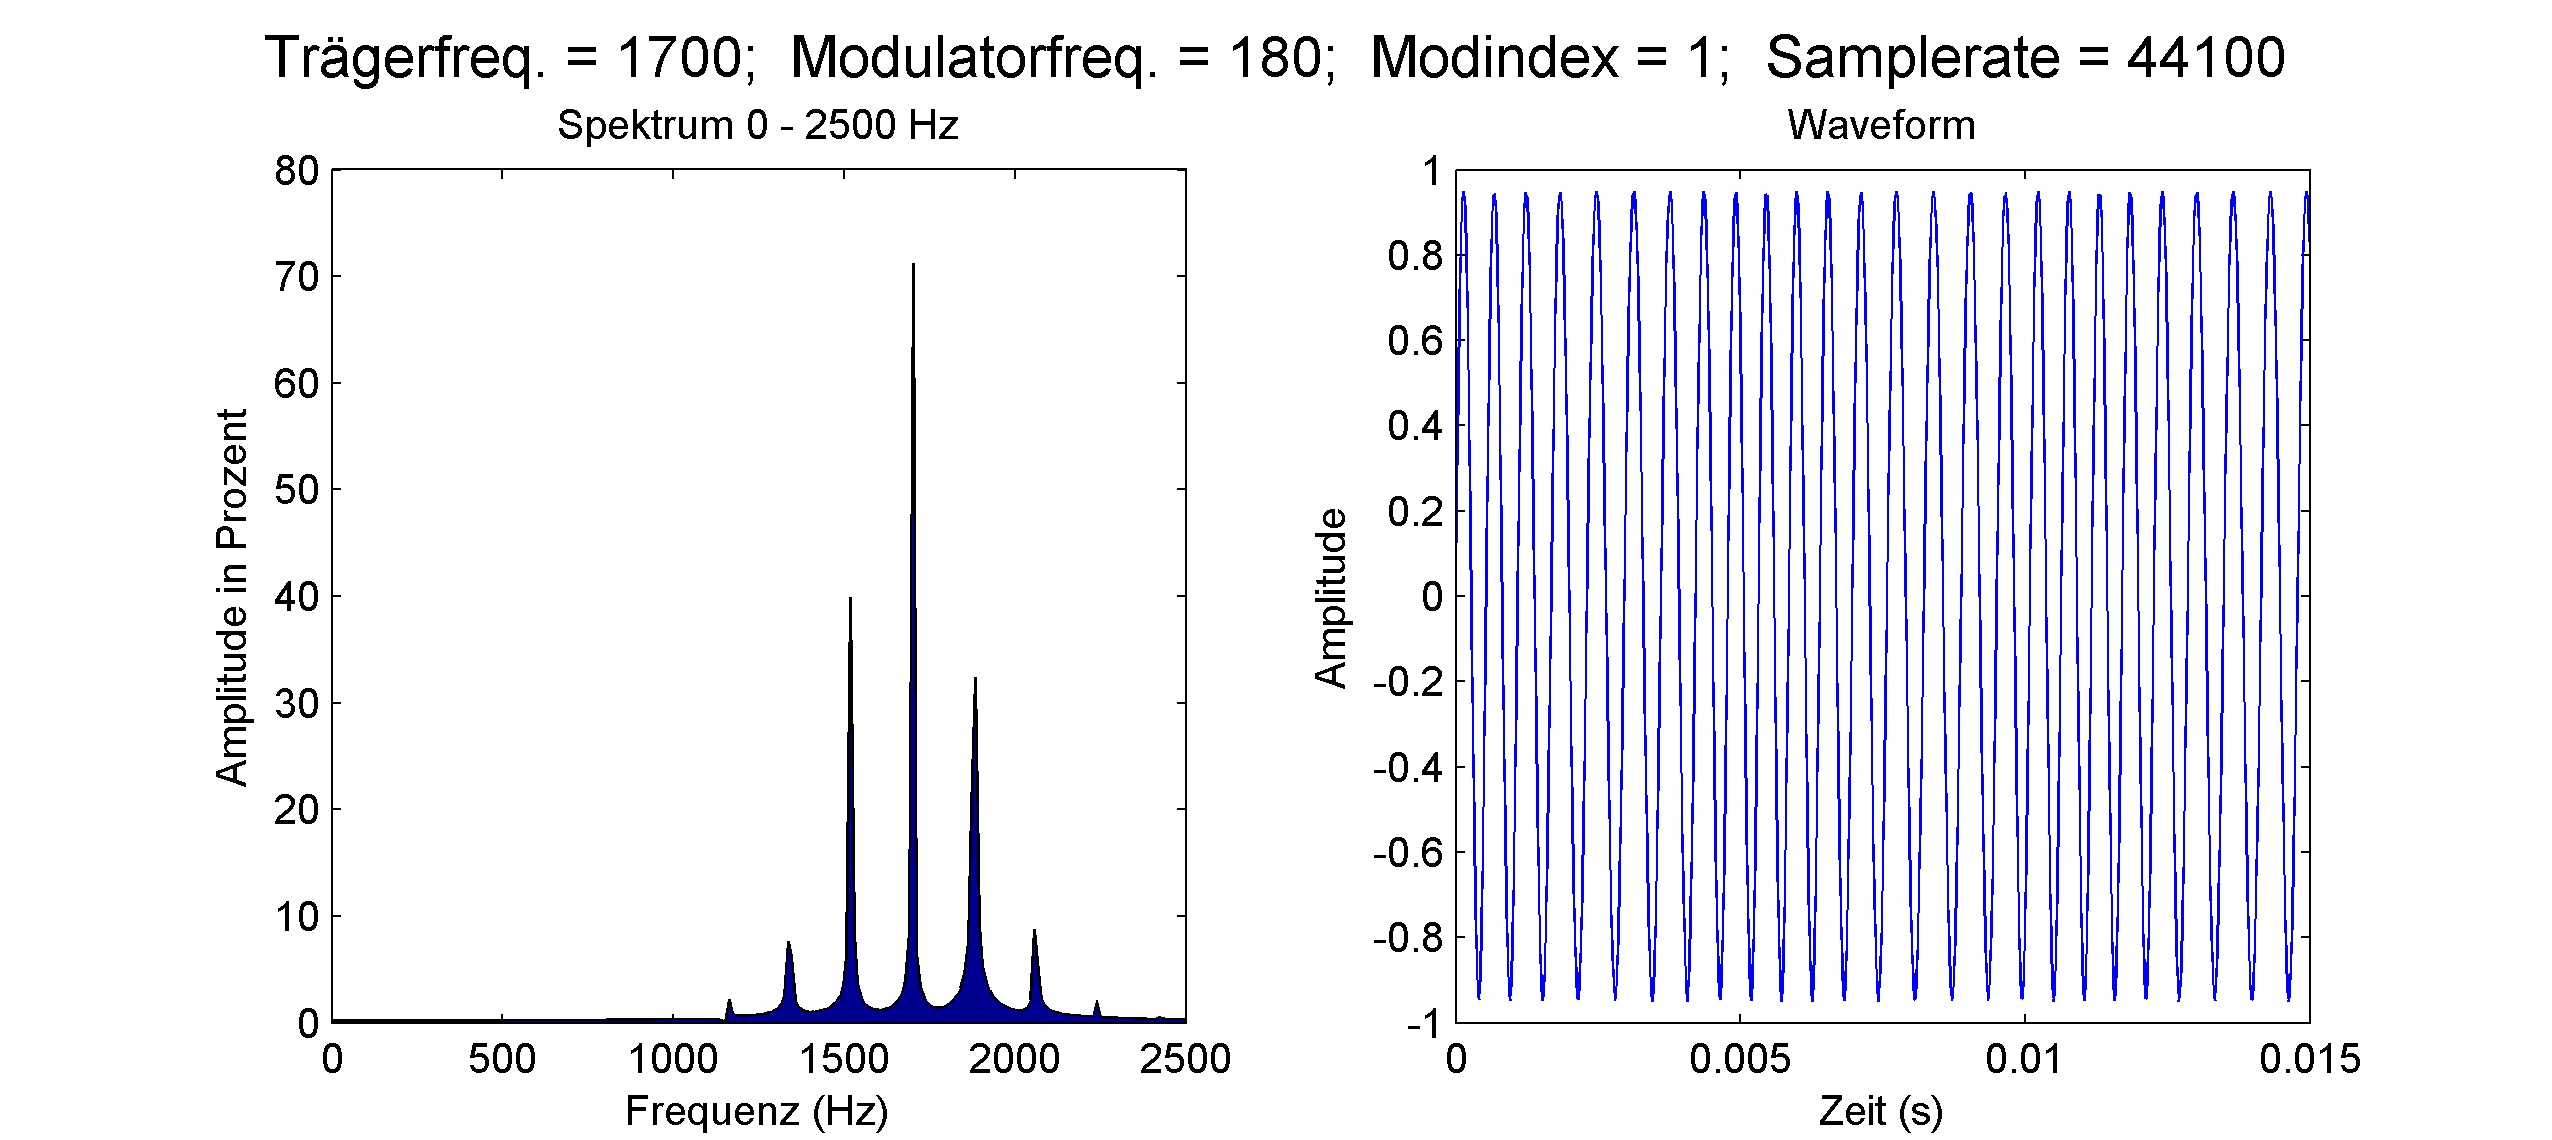
\includegraphics[width=0.95\textwidth]{par2TM.png}
\caption{Einfache FM mit $f_c = 1700$, $w_m = 180$, $I = 1$. }
Quelle: Eigene Darstellung in MATLAB
\end{figure}
\FloatBarrier
Und nun das Gesamtspektrum der Kaskadenschaltung:
\FloatBarrier
\begin{figure} [ht]
\centering
  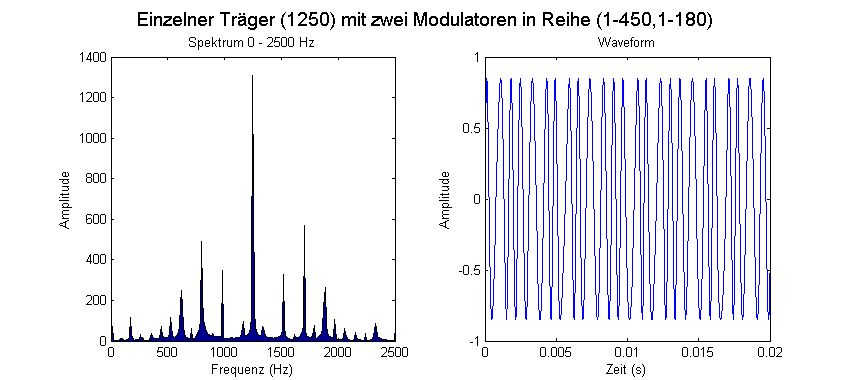
\includegraphics[width=0.95\textwidth]{kask.png}
\caption{Kaskaden-FM mit $f_c = 1250$, $w_{m1} = 450$, $w_{m2} = 180$, $I_1 = 1$, $I_2 = 1$. }
Quelle: Eigene Darstellung in MATLAB
\end{figure}
\FloatBarrier
Zum Vergleich hier nochmals das Gesamtspektrum der Parallelschaltung eines Trägers mit zwei Modulatoren:
\FloatBarrier
\begin{figure} [ht]
\centering
  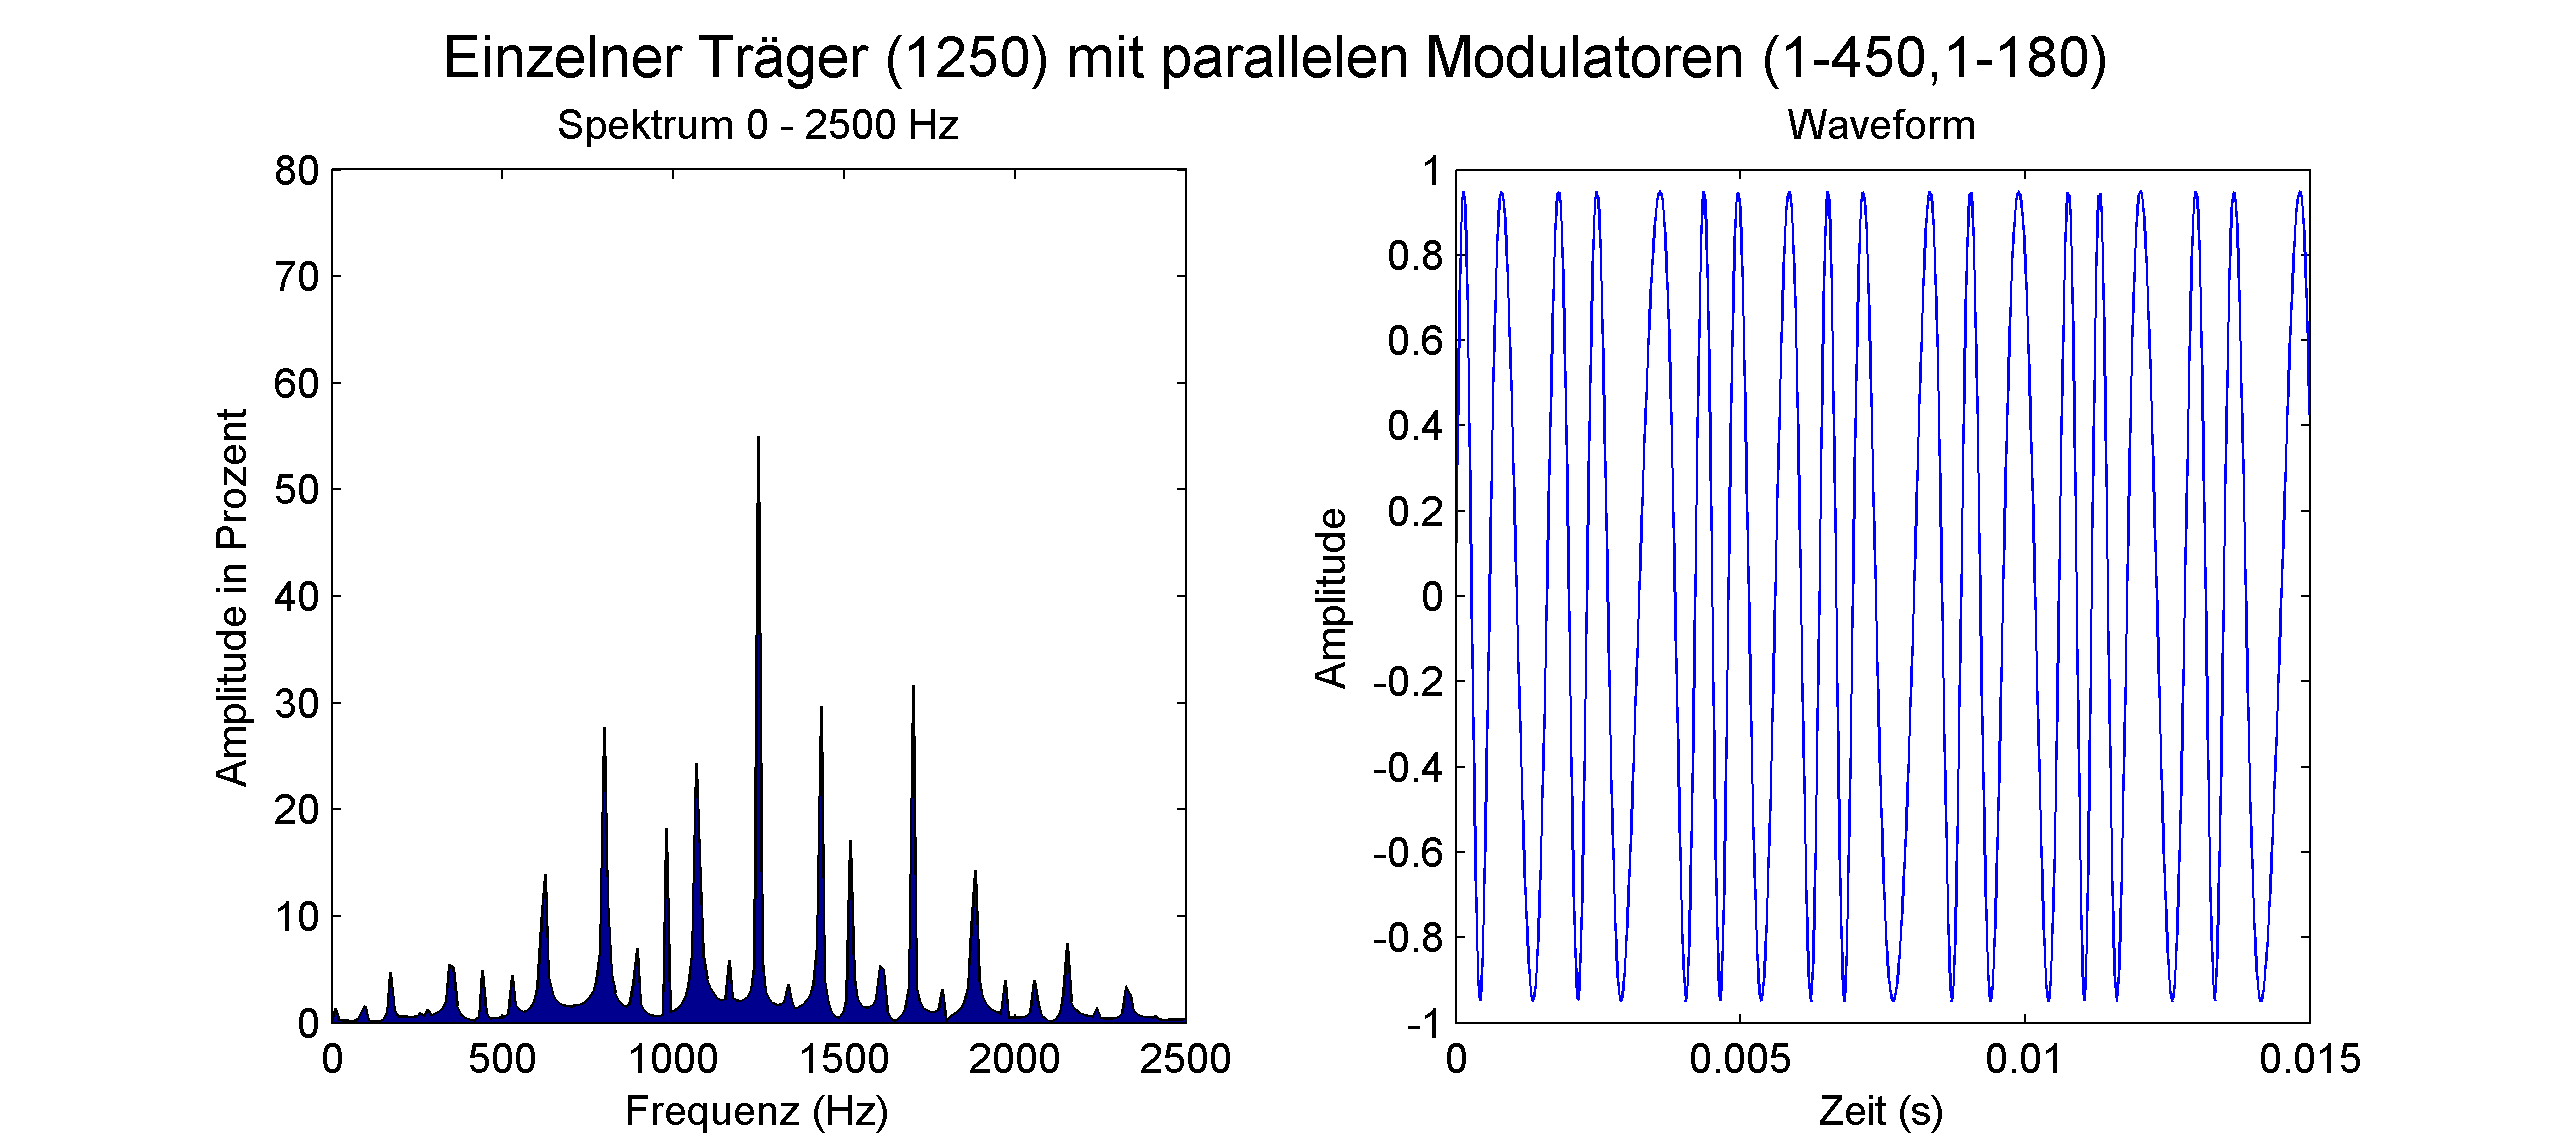
\includegraphics[width=0.95\textwidth]{parTM1M2.png}
\caption{Parallele FM mit $f_c = 1250$, $w_{m1} = 450$, $w_{m2} = 180$, $I_1 = 1$, $I_2 = 1$. }
Quelle: Eigene Darstellung in MATLAB
\end{figure}
\FloatBarrier
Die Spekten ähneln sich stark, es zeigt sich aber, dass wie erwartet die Trägerfrequenz mehr Energie erhält, da der eine Besselkoeffizient der Ordnung $0$ durch die Multiplikation des Arguments mit $0$ den Wert 1 zurückliefert, anstelle eines niedrigeren Werts wie bei der Parallelschaltung. Auch fällt auf, dass alle Nicht-Kombinationsseitenfrequenzen des äußeren Modulators entfallen (also alle Kombinationen, wo der Besselkoeffizient des inneren Modulators $M1$ die Ordnung $0$ besitzt). Dies liegt ebenfalls an der der Multiplikation von $I_2$ mit $n$, siehe \ref{Kaskadenspecials}. 

Der Vergleich wird nochmals wiederholt mit den Einstellungen $I_1 = 2$ und $I_2 = 3$. Zuerst wieder die Kaskadenschaltung:
\FloatBarrier
\begin{figure} [ht]
\centering
  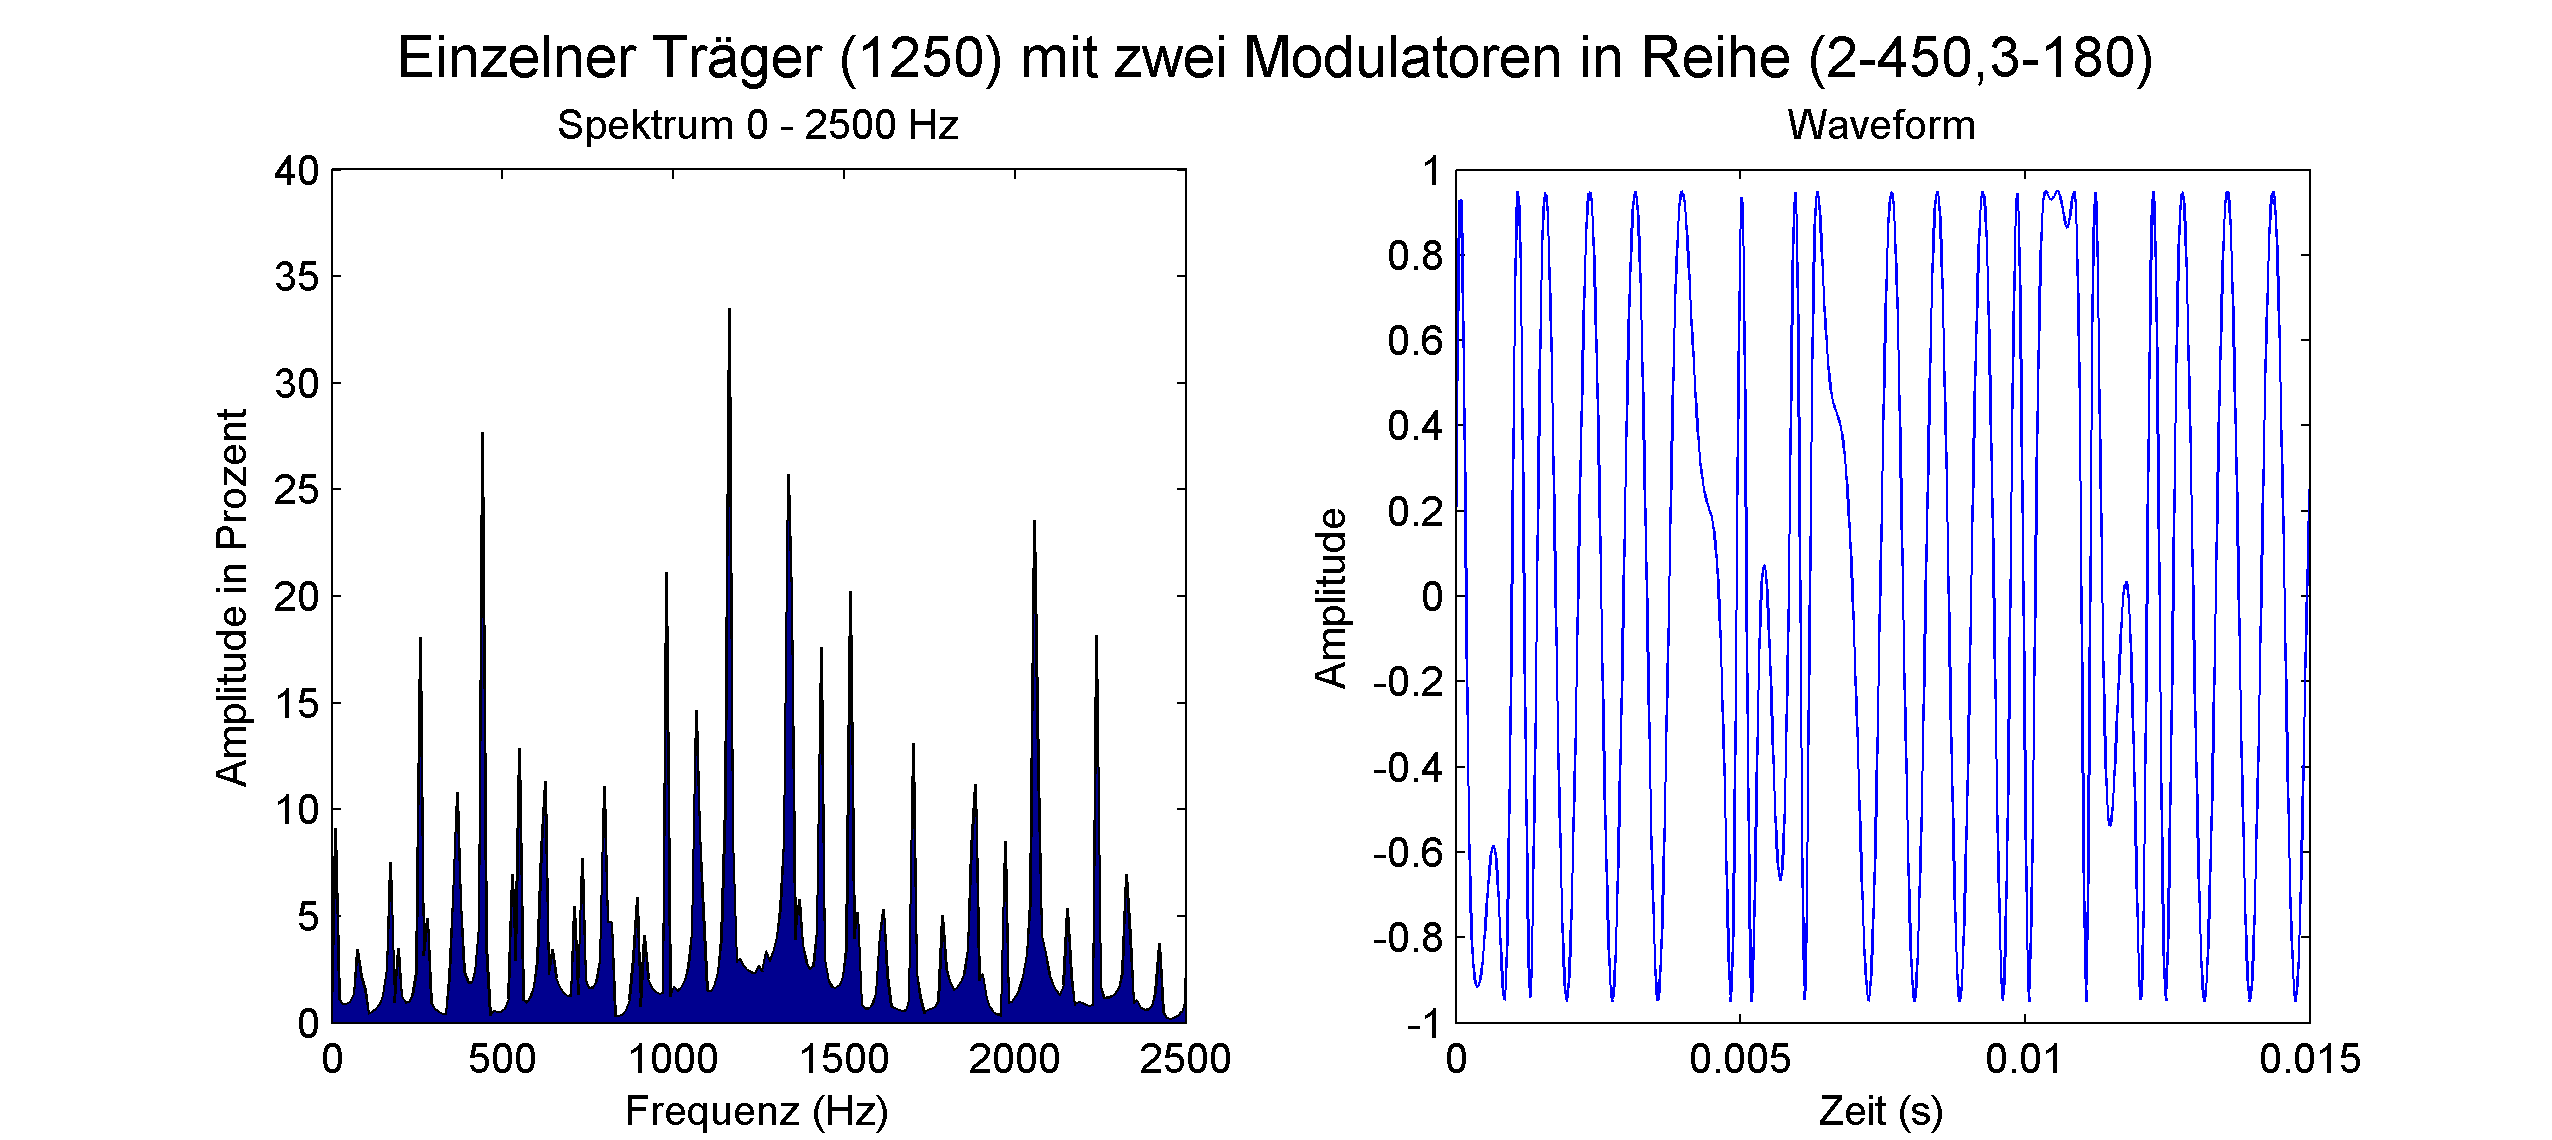
\includegraphics[width=0.95\textwidth]{kask2.png}
\caption{Kaskaden-FM mit $f_c = 1250$, $w_{m1} = 450$, $w_{m2} = 180$, $I_1 = 2$, $I_2 = 3$. }
Quelle: Eigene Darstellung in MATLAB
\end{figure}
\FloatBarrier
Und die Parallelschaltung mit zwei Modulatoren auf denselben Träger:
\FloatBarrier
\begin{figure} [ht]
\centering
  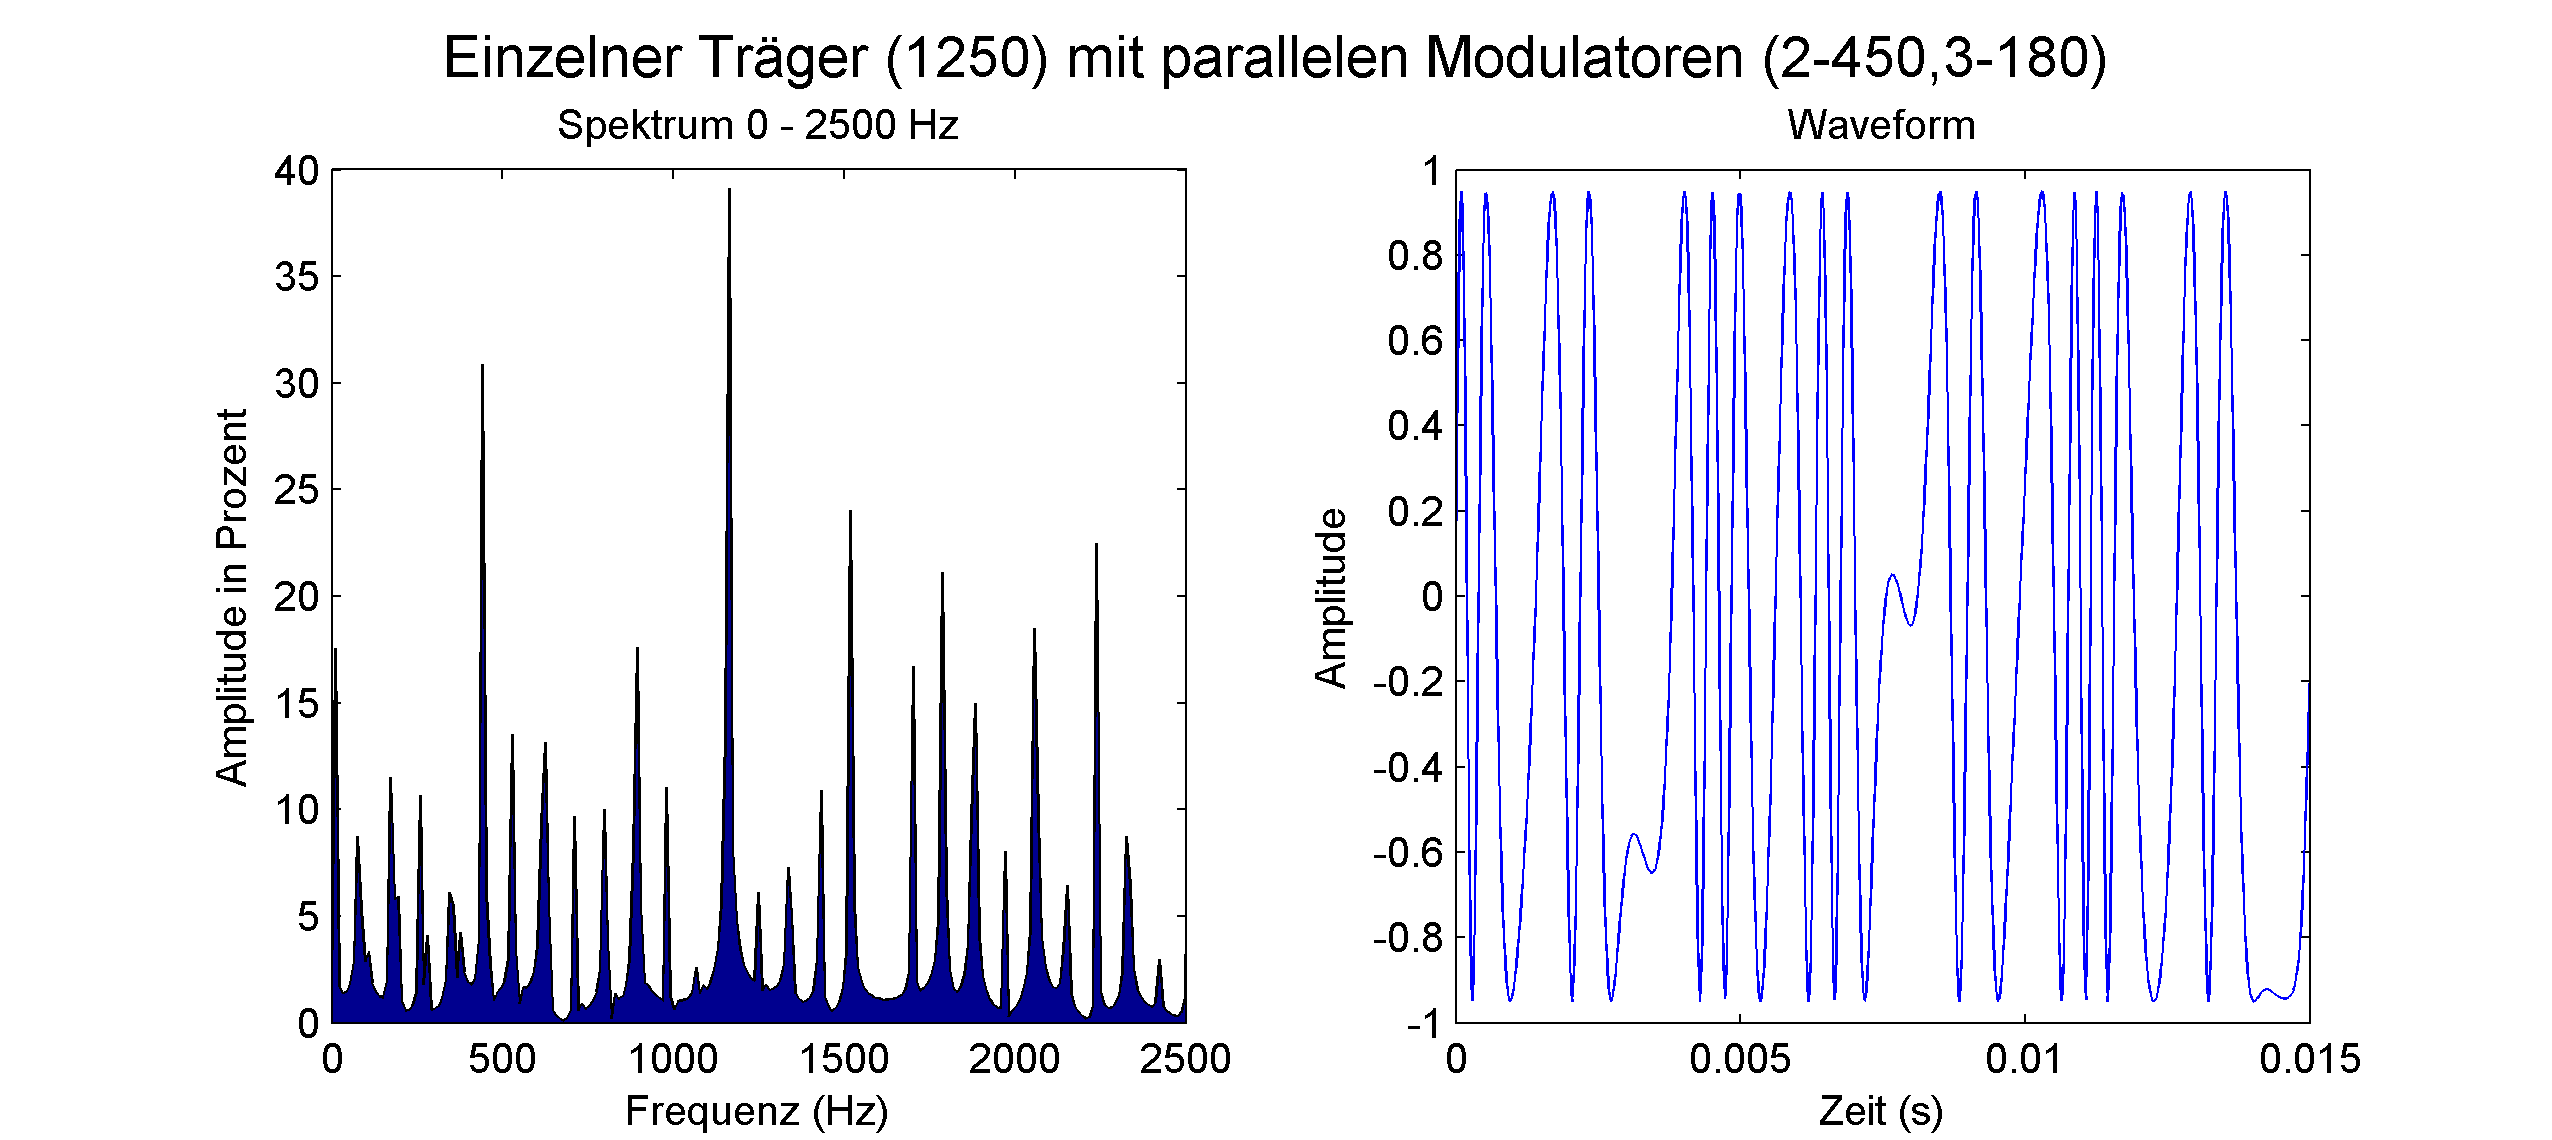
\includegraphics[width=0.95\textwidth]{parkask2.png}
\caption{Parallele FM mit $f_c = 1250$, $w_{m1} = 450$, $w_{m2} = 180$, $I_1 = 2$, $I_2 = 3$. }
Quelle: Eigene Darstellung in MATLAB
\end{figure}
\FloatBarrier
Da ein höherer Modulationsindex grundsätzlich die Bandbreite erhöht und für ein reicheres Spektrum erzeugt \cite{chowningPaper}, lassen sich schon für die gewählten Indizes von $2$ und $3$ rein visuell die Unterschiede zwischen der parallelen Modulation eines Trägers sowie der Kaskadenschaltung kaum noch nachvollziehen. Dennoch sind natürlich dieselben Prinzipien am Werk wie im vorherigen Beispiel.

\subsection{Feedbackschaltung}

Eine Spezialform der komplexen FM besteht darin, das Ausgangssignal des Trägers zur Modulation des Trägers heranzuziehen anstelle eines Modulators wie in der einfachen FM. Die Formel für eine Feedbackschaltung kann rekursiv wie folgt angegeben werden:
\begin{equation}
f_{FMfeedback}(t_{n}) = sin(w_{c}t_{n} + If_{FMfeedback}(t_{n-1})) \quad \text{mit} \quad f_{FMfeedback}(t_{n_0}) = 0
\end{equation}
In MATLAB oder in einer beliebigen Programmiersprache kann diese Formel dann natürlich komfortabel iterativ oder rekursiv implementiert werden.
Das Frequenzspektrum berechnet sich \cite{schottiWeb} über:
\begin{equation}
f_{FMfeedback}(t) = \sum_{n=1}^{\infty}\frac{2}{nI}J_n(nI)\sin{nw_{c}t}
\end{equation}
Man sieht sofort, dass die Einflussnahme auf die Feedbackschaltung durch den Modulationsindex (d.h. die Amplitude, mit der man dem Ausgangssignal der Schaltung erlaubt, auf sich selbst zurückzuwirken) lediglich die Steilheit des Abfallens der Energie von den näher am Träger liegenden Seitenbändern zu den weiter außen liegenden beeinflusst. Die Variable $n$ hängt dabei nur von der Ordnung der Besselfunktion ab und durchläuft in jedem Fall ganzzahlig die Werte von 1 bis $\infty$. In jedem Fall ist die Lage der Seitenfrequenzbänder also immer ein ganzzahliges Vielfaches der Trägerfrequenz. Der Amplitudenabfall von Band zu Band erfolgt dabei bei konstantem Modulationsindex, und wenn man die Einflussnahme von $n$ auf das Argument an die Besselfunktion und somit den Wert dieser herausrechnet, im Verhältnis $\frac{1}{2}$ zu $\frac{1}{3}$ zu $\frac{1}{4}$ zu $\frac{1}{5}$ etc. Damit weist er Ähnlichkeit zum Spektrum einer Sägezahnwelle auf, bei der die Obertöne in genau in diesen Verhältnissen zum Grundton stehen. Feedback-FM bietet damit die Möglichkeit, mit nur einem Operator Töne zu erzeugen, die einen rauen Charakter aufweisen. 

Im Folgenden sehen wir das Spektrum einer einfachen Feedbackschaltung eines Trägers, der sich selbst moduliert; einmal mit Trägerfrequenz von $220$, einmal mit Trägerfrequenz von $440$:
\FloatBarrier
\begin{figure} [ht]
\centering
  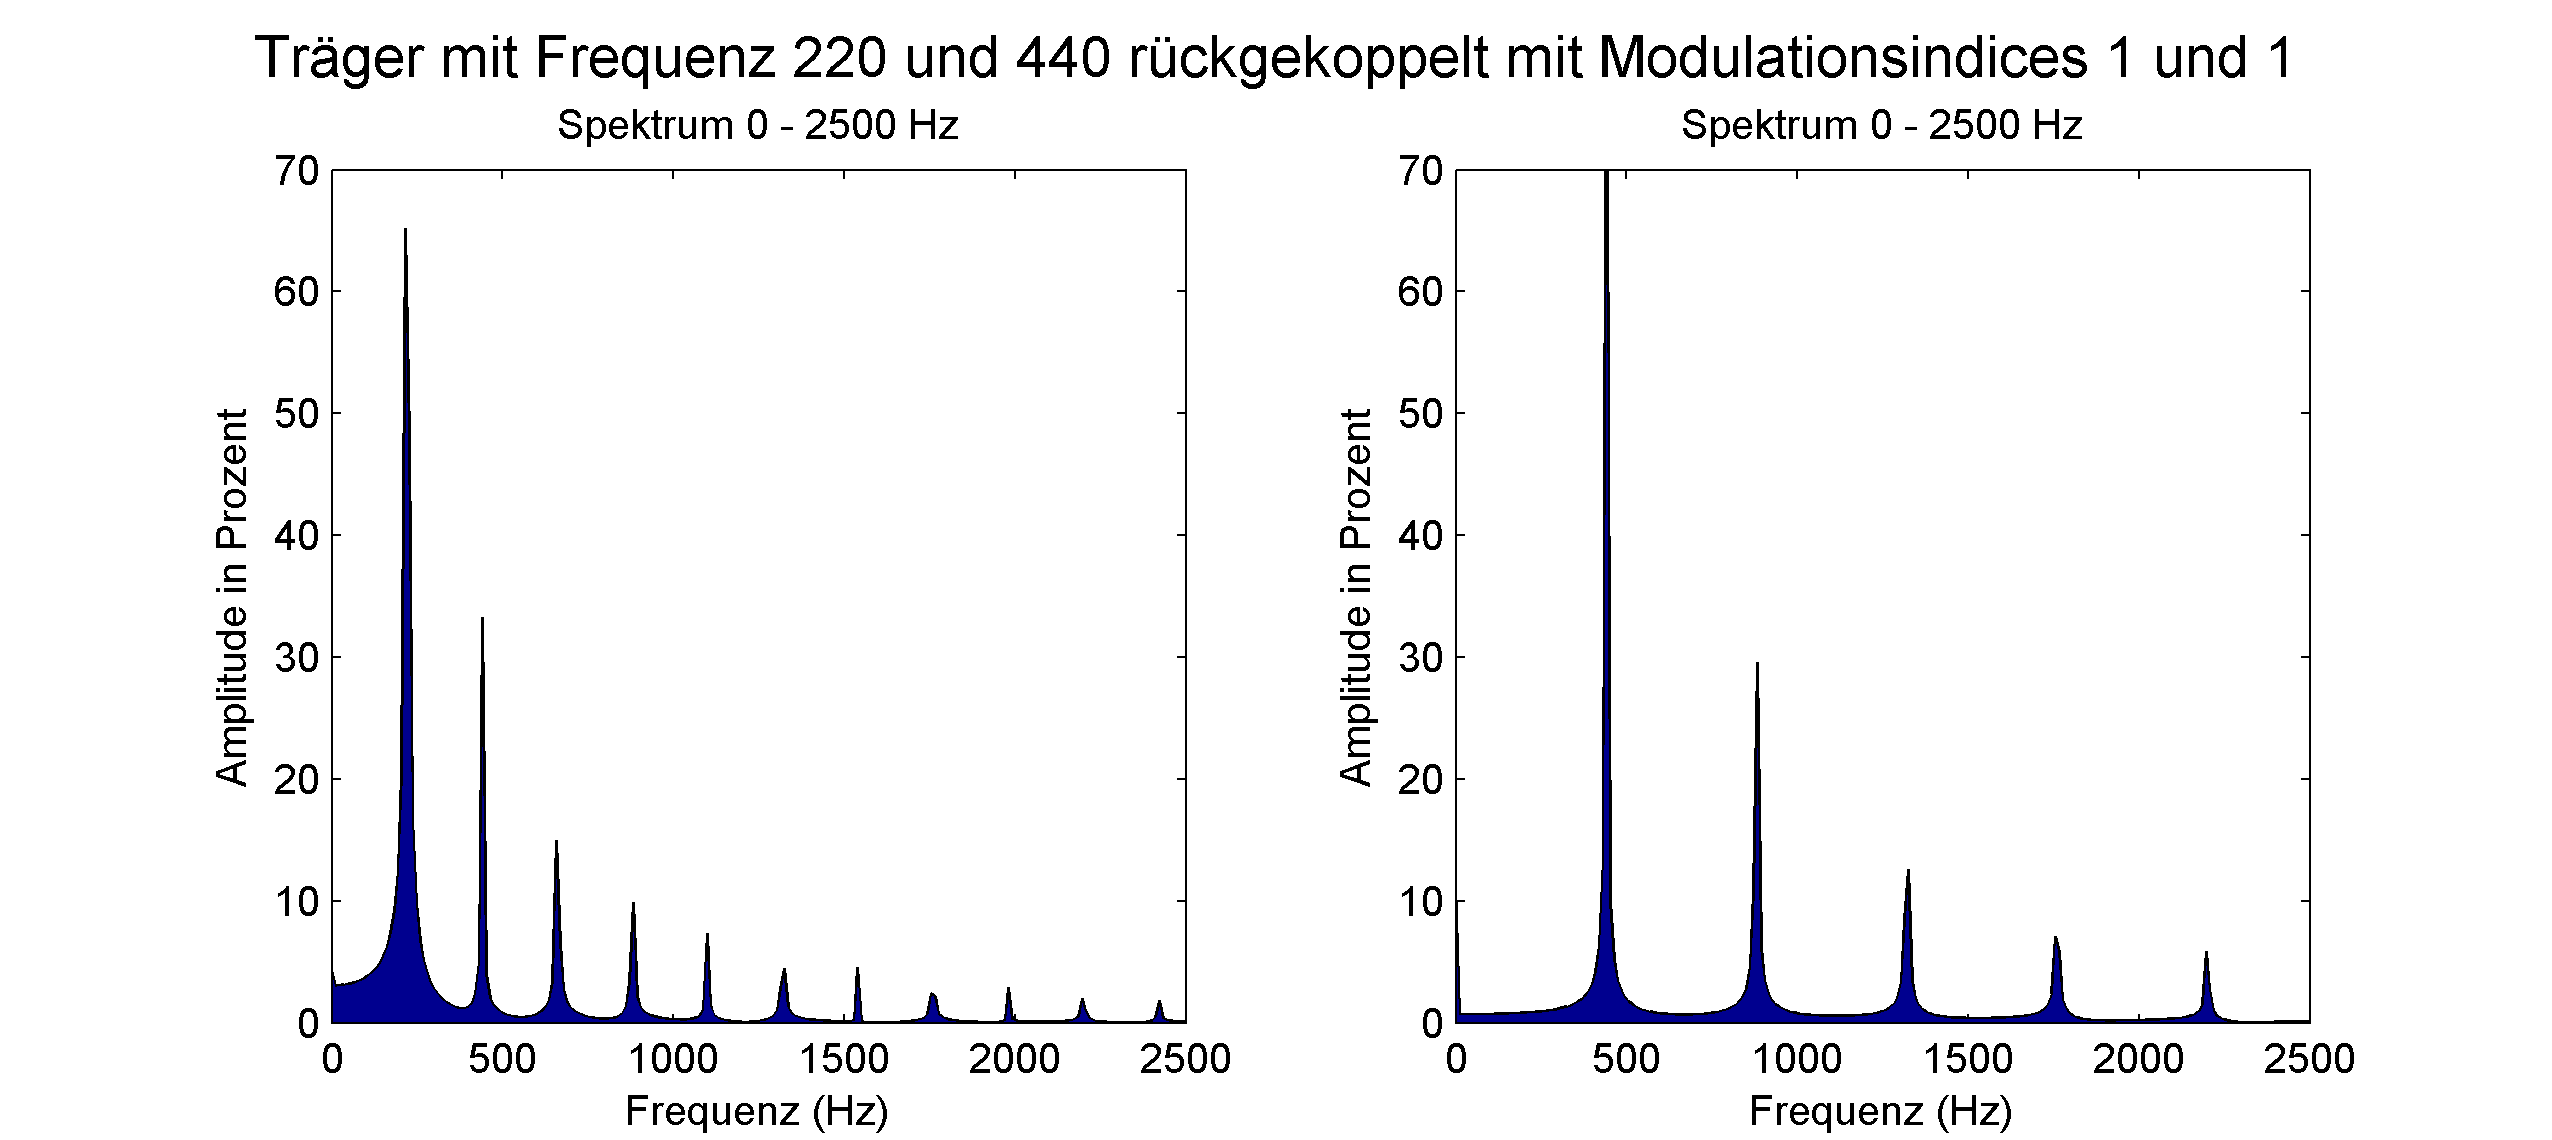
\includegraphics[width=0.95\textwidth]{feedback1.png}
\caption{Feedback-FM mit $f_{c1} = 220$, $f_{c2} = 440$, $I_1 = 1$, $I_2 = 1$. }
Quelle: Eigene Darstellung in MATLAB
\end{figure}
\FloatBarrier
Man erkennt, dass jedes Frequenzband exakt um ein Vielfaches der Trägerfrequenz von dieser entfernt liegt. Im Vergleich hier das Spektrum zweier Feedbackschaltungen mit gleicher Trägerfrequenz, einmal mit Modulationsindex von $0.5$, einmal mit Modulationsindex von $1.5$:
\FloatBarrier
\begin{figure} [ht]
\centering
  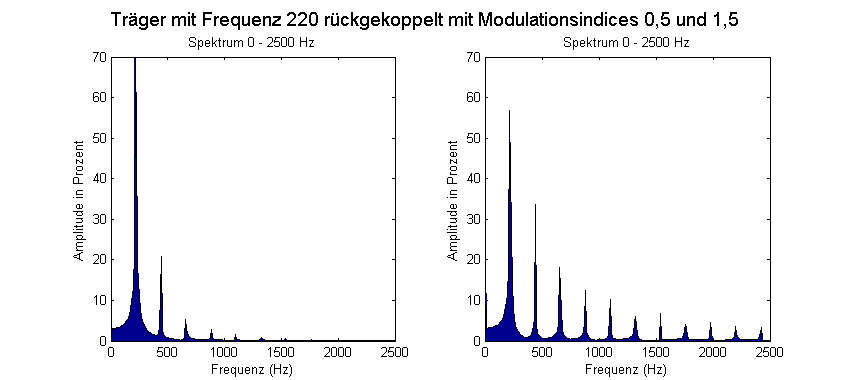
\includegraphics[width=0.95\textwidth]{feedback2.png}
\caption{Parallele FM mit $f_{c1} = 220$, $f_{c2} = 220$, $I_1 = 0.5$, $I_2 = 1.5$. }
Quelle: Eigene Darstellung in MATLAB
\end{figure}
\FloatBarrier
Man erkennt, dass sich mit steigendem Feedback das Abfallen der Seitenbänder vom Träger verlangsamt.